% ============================================================================
%  BTP Report — SRAM-Fused Triton Kernel for MC Inventory Optimisation
%  IIT Kharagpur  |  Compact edition (target: 25-30 pages)
% ============================================================================
\documentclass[11pt, a4paper, oneside]{report}

% --- Core packages ----------------------------------------------------------
\usepackage[utf8]{inputenc}
\usepackage[T1]{fontenc}
\usepackage{lmodern}
\usepackage[margin=1in]{geometry}
\usepackage{setspace}
\setstretch{1.3}

\usepackage{amsmath, amssymb, amsfonts}
\usepackage{bm}
\usepackage{graphicx}
\usepackage{booktabs}
\usepackage{array}
\usepackage{tabularx}
\usepackage{longtable}
\usepackage{float}
\usepackage{caption}
\usepackage{subcaption}
\usepackage{listings}
\usepackage{xcolor}
\usepackage{hyperref}
\usepackage{cleveref}
\usepackage{enumitem}
\usepackage{fancyhdr}
\usepackage[numbers, sort&compress]{natbib}
\usepackage{url}
\usepackage{microtype}
\usepackage{parskip}
\usepackage{tikz}
\usepackage{pgfplots}
\pgfplotsset{compat=1.18}
\usetikzlibrary{positioning, arrows.meta, calc, patterns, fit, shapes.geometric, decorations.pathreplacing}

% --- Compact chapter/section titles -----------------------------------------
\usepackage{titlesec}
\titleformat{\chapter}[display]{\normalfont\Large\bfseries}{\chaptertitlename\ \thechapter}{8pt}{\LARGE}
\titlespacing*{\chapter}{0pt}{-20pt}{12pt}
\titlespacing*{\section}{0pt}{10pt}{4pt}
\titlespacing*{\subsection}{0pt}{8pt}{3pt}
\titlespacing*{\subsubsection}{0pt}{6pt}{2pt}

% --- Compact captions -------------------------------------------------------
\captionsetup{font=small, labelfont=bf, skip=4pt}

% --- Compact lists ----------------------------------------------------------
\setlist{nosep, leftmargin=1.5em}

% --- Colours ----------------------------------------------------------------
\definecolor{codeblue}{RGB}{0,102,204}
\definecolor{codegray}{RGB}{100,100,100}
\definecolor{codegreen}{RGB}{0,128,0}
\definecolor{backcolour}{RGB}{248,248,248}
\definecolor{iitkgpred}{RGB}{139,0,0}
% Figure palette
\definecolor{cpucol}{RGB}{120,144,168}
\definecolor{ptcol}{RGB}{232,168,56}
\definecolor{trcol}{RGB}{192,57,43}
\definecolor{dmem}{RGB}{70,130,180}
\definecolor{inputmem}{RGB}{100,180,220}
\definecolor{outmem}{RGB}{180,220,140}

% --- Hyperref ---------------------------------------------------------------
\hypersetup{colorlinks=true, linkcolor=iitkgpred, citecolor=codeblue, urlcolor=codeblue}

% --- Code listing style -----------------------------------------------------
\lstset{
    backgroundcolor=\color{backcolour}, basicstyle=\ttfamily\footnotesize,
    keywordstyle=\color{codeblue}\bfseries, commentstyle=\color{codegray}\itshape,
    stringstyle=\color{codegreen}, breaklines=true, frame=single,
    rulecolor=\color{codegray!30}, numbers=left, numberstyle=\tiny\color{codegray},
    xleftmargin=2em, framexleftmargin=1.5em, captionpos=b, aboveskip=6pt, belowskip=4pt,
}

% --- Header/Footer ----------------------------------------------------------
\pagestyle{fancy}
\fancyhf{}
\fancyhead[L]{\small\leftmark}
\fancyhead[R]{\small BTP Report}
\fancyfoot[C]{\thepage}
\renewcommand{\headrulewidth}{0.4pt}

% --- Graphics path ----------------------------------------------------------
\graphicspath{{diagrams/}{report_figures/}}

% --- Boxed figures globally -------------------------------------------------
\usepackage{float}
\floatstyle{boxed}
\restylefloat{figure}

% --- Custom commands --------------------------------------------------------
\newcommand{\E}{\mathbb{E}}
\newcommand{\R}{\mathbb{R}}
\newcommand{\tflops}{\text{TFLOPS}}
\newcommand{\blockm}{\texttt{BLOCK\_M}}
\newcommand{\blockn}{\texttt{BLOCK\_N}}
\newcommand{\blockk}{\texttt{BLOCK\_K}}

% ============================================================================
\begin{document}

% --- Title page -------------------------------------------------------------
\begin{titlepage}
\centering

\vspace*{0.5cm}

{\fontsize{26}{42}\selectfont\bfseries SRAM-Fused Triton Kernels for Monte-Carlo Inventory Optimisation}

\vspace{1.2cm}

{\large\bfseries BTP PROJECT REPORT}

\vspace{0.8cm}

{\large Submitted by}\\[0.2cm]
{\large\bfseries Abhijit Kumar}\\[0.15cm]
{\large\bfseries B.Tech.\ in Industrial and Systems Engineering}\\[0.15cm]
{\large\bfseries Indian Institute of Technology Kharagpur}

\vspace{0.8cm}

{\large Under the Supervision of}\\[0.2cm]
{\large\bfseries Dr.\ ABHISHEK SHARMA}\\[0.15cm]
{\large\bfseries Department of Industrial and Systems Engineering}\\[0.15cm]
{\large\bfseries Indian Institute of Technology Kharagpur}

\vspace{0.8cm}


\includegraphics[width=3cm]{iitkgp_logo.png}

\vspace{1.5cm}

{\large\bfseries Department of Industrial \& Systems Engineering}\\[0.15cm]
{\large\bfseries Indian Institute of Technology Kharagpur}

\vspace{0.3cm}

{\large\bfseries Spring 2025--26 Session}

\vfill

\end{titlepage}

% --- Certificate from the Candidate ----------------------------------------
\newpage
\thispagestyle{empty}

\begin{center}
{\Large\bfseries\underline{CERTIFICATE FROM THE CANDIDATE}}
\end{center}

\vspace{1.5cm}

\noindent I hereby certify that the BTP/MTP project report entitled, `\textbf{SRAM-Fused Triton Kernel for Monte-Carlo Inventory Optimisation}' and submitted is completely original and has not been submitted for award of any degree/internship anywhere.

\vspace{4cm}

\noindent Yours Sincerely,

\vspace{1.5cm}

\noindent\textbf{Name:} Abhijit Kumar\\[0.3cm]
\textbf{Affiliation:} Indian Institute of Technology Kharagpur\\[0.3cm]
\textbf{Degree Programme (with batch year):} B.\ Tech.\ in Industrial\\
and Systems Engineering (2022 -- 2026)

\vspace{2cm}

\hfill\textbf{Sign.\ (with date)}

% --- Certificate from the Supervisor ---------------------------------------
\newpage
\thispagestyle{empty}

\begin{center}
{\Large\bfseries\underline{CERTIFICATE FROM THE SUPERVISOR}}
\end{center}

\vspace{1.5cm}

\noindent I hereby certify that the thesis/project report entitled, ``\textbf{SRAM-Fused Triton Kernel for Monte-Carlo Inventory Optimisation}'', which is being submitted by \textbf{Mr.\ Abhijit Kumar} for the award of \textbf{BTP} is completely original and has not been submitted for award of any degree/internship anywhere. The entire work was done under my supervision and guidance.

\vspace{6cm}

\noindent Yours Sincerely,\\
Dr.\ Abhishek Sharma\\
(Supervisor)

% --- Front matter -----------------------------------------------------------
\pagenumbering{roman}
\chapter*{Abstract}
\addcontentsline{toc}{chapter}{Abstract}
This thesis presents a high-performance GPU computing solution for the Multi-Echelon Stochastic Newsvendor Problem applied to heavy-machinery dealership networks. The classical newsvendor model, which determines optimal order quantities under stochastic demand by balancing underage costs against overage costs, is extended to a multi-echelon setting with spatially correlated demand across 2,048 product-location nodes and 131,072 Monte-Carlo scenarios. The dealership network comprises two product categories---tractors and generators---with demand correlations extracted from the M5 Kaggle forecasting dataset's hierarchical structure.

The central contribution is a custom SRAM-fused Triton kernel that eliminates the materialisation of the large intermediate demand matrix (1.0\,GB in single precision) by fusing the matrix multiplication with the newsvendor business logic entirely within on-chip SRAM. In standard frameworks such as PyTorch, the demand matrix $\mathbf{D} = \bm{\mu} + \mathbf{L}\mathbf{Z}$ must round-trip through High-Bandwidth Memory (HBM)---the dominant memory bottleneck. Inspired by FlashAttention, the proposed kernel computes demand, sales, overage, and profit within SRAM tiles, writing only the 8\,KB expected profit vector via atomic accumulation.

Three solver backends---CPU-NumPy, \texttt{torch.compile}-optimised PyTorch, and the proposed Triton-Fused kernel---are benchmarked on an NVIDIA T4 GPU. The Triton kernel achieves a \textbf{49.4\% reduction in peak GPU memory} (2.024\,GB $\to$ 1.024\,GB) and a ${\sim}40\times$ speedup over the CPU baseline. Extension kernels---which fuse more work per matmul tile---achieve 1.3--1.7$\times$ speedup over \texttt{torch.compile} with up to 90\% memory reduction (CVaR). Numerical validation confirms agreement within floating-point tolerance (maximum absolute deviation $< 0.005$).

A four-stage ETL pipeline hybridises real M5 spatial correlations (auto-downloaded via \texttt{kagglehub}) with realistic heavy-machinery financial parameters. Nine autotune configurations targeting the T4's 48\,KB SRAM budget ensure portability across GPU architectures. Four extensions demonstrate the paradigm's generality: (i)~optimal $Q^*$ grid search with single-matmul fusion (+5.3\% aggregate profit improvement), (ii)~CVaR risk evaluation with fused histogram accumulation (identifying 17.5$\times$ higher tail risk in generators), (iii)~budget-constrained optimisation via Lagrangian bisection (converging in 13 iterations), and (iv)~multi-product demand substitution with a two-pass kernel architecture (+10.3\% aggregate profit).

\vspace{0.8em}
\noindent\textbf{Keywords:} Monte-Carlo simulation, Newsvendor problem, GPU computing, Triton, kernel fusion, SRAM optimisation, inventory management, stochastic optimisation, multi-echelon supply chain, high-performance computing.


\tableofcontents
\listoffigures
\listoftables

\chapter*{List of Abbreviations}
\addcontentsline{toc}{chapter}{List of Abbreviations}
\vspace{-0.5em}
\begin{longtable}{@{} >{\bfseries}l l @{}}
\toprule
\textbf{Abbreviation} & \textbf{Full Form} \\
\midrule
\endhead
CPU / GPU  & Central / Graphics Processing Unit \\
CUDA       & Compute Unified Device Architecture \\
CVaR / VaR & Conditional Value at Risk / Value at Risk \\
ETL        & Extract, Transform, Load \\
FP32       & 32-bit Floating Point (Single Precision) \\
HBM        & High-Bandwidth Memory \\
JIT        & Just-In-Time Compilation \\
MC / SAA   & Monte-Carlo / Sample Average Approximation \\
SM         & Streaming Multiprocessor \\
SRAM       & Static Random-Access Memory \\
TFLOPS     & Tera Floating-Point Operations Per Second \\
\bottomrule
\end{longtable}


% --- Main matter ------------------------------------------------------------
\pagenumbering{arabic}

\chapter{Introduction}\label{ch:intro}
\section{Background}\label{sec:background}

Inventory management is a critical operational decision in manufacturing and retail~\citep{silver2017}. The \emph{Newsvendor Problem}~\citep{arrow1951, porteus2002} formalises the trade-off between under-ordering (lost sales) and over-ordering (excess inventory) under stochastic demand. In practice, modern supply chains are multi-echelon, with spatially correlated demand across nodes~\citep{clark1960, graves2000}. Ignoring these correlations leads to suboptimal ordering policies and profit erosion.

\section{Problem Statement}\label{sec:problem}

This thesis addresses the Multi-Echelon Stochastic Newsvendor Problem for a dealership network of tractors and generators across $N = 2{,}048$ nodes with $S = 131{,}072$ Monte-Carlo scenarios. The intermediate demand matrix $\mathbf{D} = \bm{\mu} + \mathbf{L}\mathbf{Z}$ occupies ${\sim}1.07$\,GB in FP32, creating a memory bandwidth bottleneck~\citep{ivanov2021} when materialised in HBM by standard frameworks like PyTorch~\citep{paszke2019}.

\section{Motivation and Objectives}\label{sec:motivation}

Inspired by FlashAttention's~\citep{dao2022} strategy of fusing matmul with downstream operations within SRAM, we apply kernel fusion to inventory optimisation. The objectives are: (i)~design a custom Triton kernel fusing demand generation, newsvendor profit, and reduction into a single pass; (ii)~develop a realistic data pipeline using M5 dataset~\citep{makridakis2022} correlations; (iii)~benchmark against CPU-NumPy and \texttt{torch.compile} baselines; (iv)~develop four extensions (grid search, CVaR, budget, substitution); (v)~demonstrate GPU portability via autotuning.

\section{System Architecture}\label{sec:sysarch}

The system comprises five modules (\Cref{fig:sysarch}): centralised configuration, a four-stage ETL pipeline, two baseline solvers, the fused Triton kernel, and a benchmarking suite.

\begin{figure}[H]
\centering
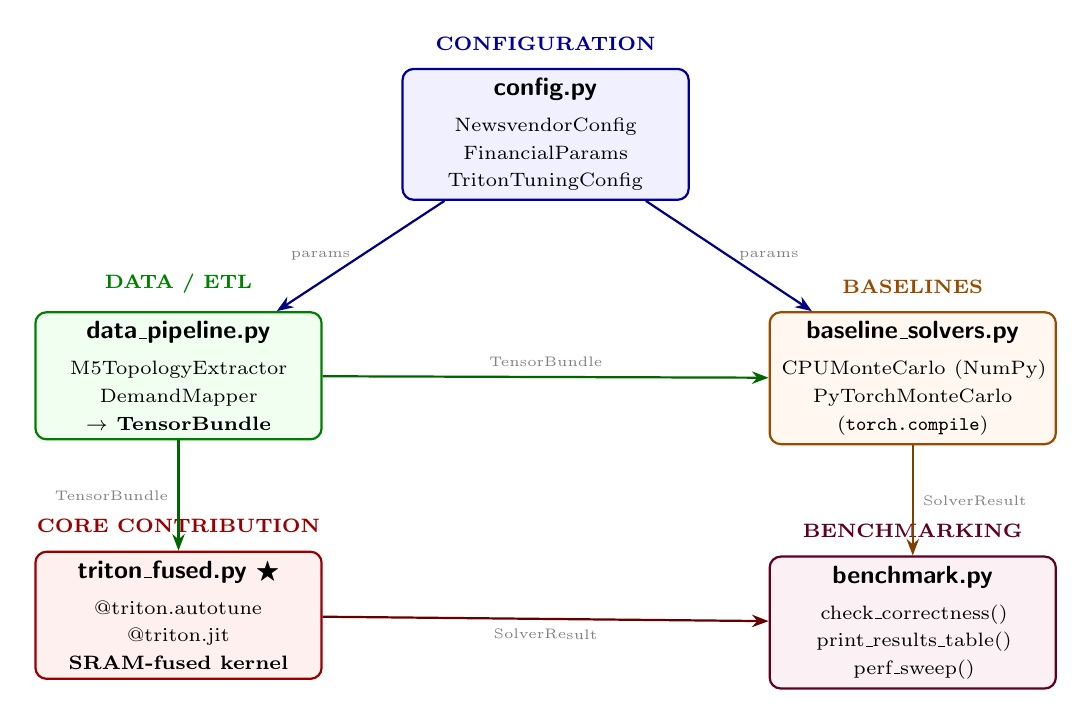
\begin{tikzpicture}[node distance=1.2cm and 1.8cm, font=\small]

% --- Styles (no #1 to avoid Beamer-like issues) ---
\tikzset{
    modbox/.style={rectangle, rounded corners=4pt, minimum width=3.6cm, minimum height=1.4cm, align=center, thick, text width=3.4cm},
}

% --- Row 1: Config (top centre) ---
\node[modbox, draw=blue!60!black, fill=blue!6] (cfg) {
    \textbf{\textsf{config.py}}\\[2pt]
    {\scriptsize NewsvendorConfig}\\[-1pt]
    {\scriptsize FinancialParams}\\[-1pt]
    {\scriptsize TritonTuningConfig}
};
\node[font=\scriptsize\bfseries, text=blue!60!black, above=0.1cm of cfg] {CONFIGURATION};

% --- Row 2: Pipeline (left) and Baselines (right) ---
\node[modbox, draw=green!50!black, fill=green!6, below left=1.4cm and 1.0cm of cfg] (pipe) {
    \textbf{\textsf{data\_pipeline.py}}\\[2pt]
    {\scriptsize M5TopologyExtractor}\\[-1pt]
    {\scriptsize DemandMapper}\\[-1pt]
    {\scriptsize $\to$ \textbf{TensorBundle}}
};
\node[font=\scriptsize\bfseries, text=green!50!black, above=0.1cm of pipe] {DATA / ETL};

\node[modbox, draw=orange!60!black, fill=orange!6, below right=1.4cm and 1.0cm of cfg] (base) {
    \textbf{\textsf{baseline\_solvers.py}}\\[2pt]
    {\scriptsize CPUMonteCarlo (NumPy)}\\[-1pt]
    {\scriptsize PyTorchMonteCarlo}\\[-1pt]
    {\scriptsize (\texttt{torch.compile})}
};
\node[font=\scriptsize\bfseries, text=orange!60!black, above=0.1cm of base] {BASELINES};

% --- Row 3: Triton (left) and Benchmark (right) ---
\node[modbox, draw=red!60!black, fill=red!6, below=1.4cm of pipe] (triton) {
    \textbf{\textsf{triton\_fused.py}} $\bigstar$\\[2pt]
    {\scriptsize @triton.autotune}\\[-1pt]
    {\scriptsize @triton.jit}\\[-1pt]
    {\scriptsize \textbf{SRAM-fused kernel}}
};
\node[font=\scriptsize\bfseries, text=red!60!black, above=0.1cm of triton] {CORE CONTRIBUTION};

\node[modbox, draw=purple!50!black, fill=purple!6, below=1.4cm of base] (bench) {
    \textbf{\textsf{benchmark.py}}\\[2pt]
    {\scriptsize check\_correctness()}\\[-1pt]
    {\scriptsize print\_results\_table()}\\[-1pt]
    {\scriptsize perf\_sweep()}
};
\node[font=\scriptsize\bfseries, text=purple!50!black, above=0.1cm of bench] {BENCHMARKING};

% --- Arrows with labels ---
\draw[-{Stealth[length=6pt]}, thick, blue!50!black] (cfg) -- node[left, font=\tiny, text=gray] {params} (pipe);
\draw[-{Stealth[length=6pt]}, thick, blue!50!black] (cfg) -- node[right, font=\tiny, text=gray] {params} (base);

\draw[-{Stealth[length=6pt]}, thick, green!40!black] (pipe) -- node[left, font=\tiny, text=gray] {TensorBundle} (triton);
\draw[-{Stealth[length=6pt]}, thick, green!40!black] (pipe) -- node[above, font=\tiny, text=gray, sloped] {TensorBundle} (base);

\draw[-{Stealth[length=6pt]}, thick, red!40!black] (triton) -- node[below, font=\tiny, text=gray, sloped] {SolverResult} (bench);
\draw[-{Stealth[length=6pt]}, thick, orange!50!black] (base) -- node[right, font=\tiny, text=gray] {SolverResult} (bench);

\end{tikzpicture}
\caption{System architecture: module dependency graph. Arrows indicate data flow; \texttt{TensorBundle} is the universal data contract between the pipeline and all solvers.}
\label{fig:sysarch}
\end{figure}

\section{Scope and Report Organisation}\label{sec:scope}

This work focuses on the single-period newsvendor problem targeting NVIDIA GPUs (CUDA 7.0+). Multi-period models, dynamic pricing, and lead-time variability are beyond scope but discussed as future work in \Cref{ch:conclusions}. The report proceeds as follows: \Cref{ch:litreview}~(literature), \Cref{ch:method}~(data pipeline), \Cref{ch:model}~(solvers), \Cref{ch:extensions}~(extensions), \Cref{ch:results}~(results), \Cref{ch:conclusions}~(conclusions).


\chapter{Literature Review}\label{ch:litreview}
\section{Newsvendor Problem and Multi-Echelon Extensions}

The newsvendor problem~\citep{arrow1951} determines the optimal order quantity $Q^* = F^{-1}\!\left(\frac{p-c}{p-s}\right)$ for a single perishable product under stochastic demand~\citep{porteus2002}. Clark and Scarf~\citep{clark1960} extended this to multi-echelon systems, with later generalisations by Federgruen and Zipkin~\citep{federgruen1984} and Graves and Willems~\citep{graves2000}. However, analytical tractability diminishes with scale, motivating simulation-based approaches.

\section{Monte-Carlo Simulation and Correlated Demand}

Monte-Carlo methods with sample average approximation (SAA) offer flexibility for complex, correlated demand~\citep{birge2011, shapiro2014}. Spatial correlations are modelled via the Cholesky decomposition $\bm{\Sigma} = \mathbf{L}\mathbf{L}^\top$, generating correlated scenarios as $\mathbf{D} = \bm{\mu} + \mathbf{L}\mathbf{Z}$~\citep{glasserman2003}. The M5 forecasting dataset~\citep{makridakis2022} provides realistic hierarchical correlation structures across 3,049 products and 10 stores.

\section{GPU Computing and the Memory Wall}

Modern GPUs offer massive parallelism but suffer from the ``memory wall''~\citep{wulf1995}. Ivanov et al.~\citep{ivanov2021} showed that intermediate tensor materialisation dominates cost in data-intensive workloads. For the newsvendor problem, the $\mathbf{D}[N,S]$ matrix must make a round-trip through HBM, creating the primary bottleneck.

\section{Kernel Fusion, Triton, and FlashAttention}

Kernel fusion eliminates intermediate memory accesses by combining sequential GPU kernels~\citep{wang2010}. The Triton language~\citep{tillet2019} provides a Python DSL for writing custom tiled GPU kernels with autotuning. FlashAttention~\citep{dao2022, dao2023} demonstrated that fusing matmul with downstream operations within SRAM avoids materialising the $N \times N$ attention matrix---a direct analogue to our approach. PyTorch's \texttt{torch.compile}~\citep{ansel2024} can fuse element-wise operations but \emph{cannot} fuse across the cuBLAS matmul boundary, leaving the $\mathbf{D}$ matrix in HBM.

\section{Risk Measures and Related Work}

Conditional Value-at-Risk (CVaR), also known as Expected Shortfall, was formalised by Rockafellar and Uryasev~\citep{rockafellar2000} as a coherent risk measure that captures tail behaviour beyond Value-at-Risk (VaR). For a confidence level $\alpha \in (0,1)$, $\text{CVaR}_\alpha$ is defined as the expected value of the loss distribution in the worst $(1-\alpha)$ fraction of scenarios. Formally, if $\pi$ denotes profit, $\text{CVaR}_\alpha(\pi) = \mathbb{E}[\pi \mid \pi \leq q_\alpha]$, where $q_\alpha = F^{-1}(1-\alpha)$ is the $\alpha$-quantile of the profit distribution. Computing CVaR exactly requires sorting all $S$ scenario profits to identify the quantile threshold---an $O(S \log S)$ operation that is particularly expensive on GPUs, where comparison-based sorting requires multiple synchronisation barriers across thread blocks. Histogram-based approximations offer a practical alternative: by binning the profit values into $B$ equally spaced buckets and accumulating counts, the quantile can be located by scanning the cumulative histogram, reducing the problem to $O(S + B)$ with embarrassingly parallel binning. This histogram approach is well-suited to the GPU's SIMT execution model and avoids the global synchronisation overhead of sorting.

CVaR has been applied to newsvendor settings by Gotoh and Takano~\citep{gotoh2007} and Chen et al.~\citep{chen2009}, who demonstrated that risk-averse ordering policies reduce the probability of catastrophic losses at the expense of modest reductions in expected profit. Prior GPU work on inventory models focused on parallelising scenario evaluation across CUDA cores~\citep{pichitlamken2012} or accelerating the underlying linear algebra with cuBLAS~\citep{munguia2019}, but these approaches still materialise intermediate tensors in HBM. To our knowledge, fusing the demand matmul with newsvendor logic into a single SRAM-resident kernel has not been previously reported in the literature. The approach is conceptually analogous to FlashAttention's treatment of the attention score matrix as a transient intermediate, but applied to the inventory optimisation domain where the intermediate demand matrix $\mathbf{D}$ plays the analogous role.

\section{Summary of Research Gaps}

The literature reveals three key gaps that this thesis addresses.

\textbf{Gap 1: Kernel fusion for inventory optimisation.} Existing GPU-accelerated inventory models parallelise scenario evaluation across CUDA cores but still materialise intermediate tensors---most critically the demand matrix $\mathbf{D} \in \mathbb{R}^{N \times S}$---in high-bandwidth memory (HBM). This materialisation creates a round-trip memory access pattern where the demand matrix is written to HBM after the matmul and then read back for profit computation, consuming bandwidth that dominates total execution time. The kernel fusion paradigm pioneered by FlashAttention~\citep{dao2022} for transformer attention has not been applied to the inventory optimisation domain, despite the structural similarity between the transient attention-score matrix and the transient demand matrix.

\textbf{Gap 2: The \texttt{torch.compile} fusion boundary.} PyTorch's \texttt{torch.compile} with the Inductor backend~\citep{ansel2024} can fuse chains of element-wise operations into a single kernel, but it cannot fuse operations across the cuBLAS matrix multiplication boundary. The demand generation step $\mathbf{D} = \bm{\mu} + \mathbf{L}\mathbf{Z}$ invokes cuBLAS for the $\mathbf{L}\mathbf{Z}$ matmul, and the subsequent newsvendor profit logic (clamping, min/max, multiply-accumulate) is compiled into a separate kernel. This two-kernel pattern forces the full $\mathbf{D}$ matrix through HBM, negating much of the benefit of GPU parallelism for memory-bound problem sizes. Closing this gap requires a custom kernel that implements both the tiled matmul and the downstream profit arithmetic within a single SRAM-resident pass.

\textbf{Gap 3: Risk-aware and constrained GPU-fused extensions.} While CVaR-based newsvendor formulations exist in the operations research literature~\citep{gotoh2007, chen2009} and budget-constrained inventory models have been studied analytically~\citep{porteus2002}, GPU-fused implementations of these extensions have not been explored. Computing CVaR on GPU requires efficient tail-quantile estimation over millions of scenarios, and budget constraints introduce coupling across nodes that complicates parallelisation. Developing these extensions within the fused-kernel framework demonstrates both the generality of the approach and its practical relevance for risk-aware supply chain decision-making.

The Triton programming model provides the ideal platform to close these gaps, offering Python-level accessibility with hardware-level control over SRAM tiling and autotuning across GPU architectures.

The ideal solution would combine the tiled matmul capability of cuBLAS with the element-wise fusion of the Inductor backend, all within a single kernel that respects the SRAM budget of the target GPU. This is precisely what the Triton programming model enables: the developer specifies the tile dimensions and the fused computation in Python, and the Triton compiler generates machine code that manages shared memory, register allocation, and memory coalescing automatically. The resulting kernel can be autotuned across a small grid of tile configurations, yielding near-optimal performance without manual assembly-level optimisation.


\chapter{Methodology}\label{ch:method}
\section{Overview}

The methodology has four stages: (i)~correlation topology extraction, (ii)~demand distribution mapping, (iii)~financial tensor generation, and (iv)~Monte-Carlo simulation with kernel-fused profit computation (\Cref{fig:pipeline}).

\begin{figure}[H]
\centering
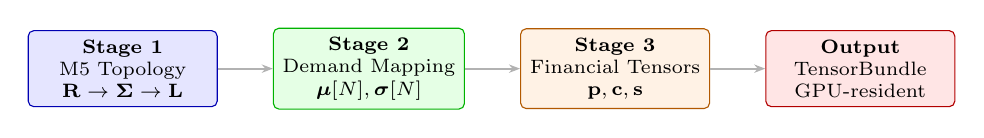
\begin{tikzpicture}[
    node distance=0.4cm and 0.5cm,
    stage/.style={rectangle, rounded corners=2pt, draw=#1!70!black, fill=#1!10, minimum width=2.4cm, minimum height=0.9cm, align=center, font=\scriptsize},
    arr/.style={-{Stealth[length=4pt]}, thick, draw=gray!60},
]
\node[stage=blue] (s1) {\textbf{Stage 1}\\M5 Topology\\$\mathbf{R} \to \bm{\Sigma} \to \mathbf{L}$};
\node[stage=green, right=0.7cm of s1] (s2) {\textbf{Stage 2}\\Demand Mapping\\$\bm{\mu}[N], \bm{\sigma}[N]$};
\node[stage=orange, right=0.7cm of s2] (s3) {\textbf{Stage 3}\\Financial Tensors\\$\mathbf{p}, \mathbf{c}, \mathbf{s}$};
\node[stage=red, right=0.7cm of s3] (s4) {\textbf{Output}\\TensorBundle\\GPU-resident};
\draw[arr] (s1) -- (s2);
\draw[arr] (s2) -- (s3);
\draw[arr] (s3) -- (s4);
\end{tikzpicture}
\caption{Four-stage ETL pipeline from raw data to GPU-resident TensorBundle.}
\label{fig:pipeline}
\end{figure}

\section{Mathematical Framework}\label{sec:math}

The expected profit for each product-location node $i$ is:
\begin{equation}\label{eq:expected-profit}
    \E[\pi_i] = \frac{1}{S} \sum_{s=1}^{S} \Big[ p_i \cdot X_{i,s} - c_i \cdot Q_i + s_i \cdot \max(Q_i - D_{i,s},\, 0) \Big],
\end{equation}
where $D_{i,s} = \max(\mu_i + \sum_k L_{ik} Z_{ks},\, 0)$, $X_{i,s} = \min(D_{i,s}, Q_i)$, $Q_i = \mu_i$, and $\mathbf{L}$ is the Cholesky factor of $\bm{\Sigma}$. The five-step computation flow is shown in \Cref{fig:mathflow}.

\begin{figure}[H]
\centering
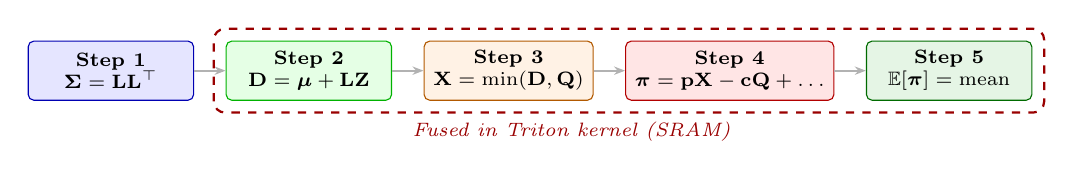
\begin{tikzpicture}[
    node distance=0.15cm and 0.35cm,
    step/.style={rectangle, rounded corners=2pt, draw=#1!70!black, fill=#1!10, minimum width=2.1cm, minimum height=0.75cm, align=center, font=\scriptsize},
    arr/.style={-{Stealth[length=4pt]}, thick, draw=gray!60},
]
\node[step=blue] (c1) {\textbf{Step 1}\\$\bm{\Sigma}=\mathbf{L}\mathbf{L}^\top$};
\node[step=green, right=0.4cm of c1] (c2) {\textbf{Step 2}\\$\mathbf{D}=\bm{\mu}+\mathbf{L}\mathbf{Z}$};
\node[step=orange, right=0.4cm of c2] (c3) {\textbf{Step 3}\\$\mathbf{X}=\min(\mathbf{D},\mathbf{Q})$};
\node[step=red, right=0.4cm of c3] (c4) {\textbf{Step 4}\\$\bm{\pi}=\mathbf{p}\mathbf{X}-\mathbf{c}\mathbf{Q}+\ldots$};
\node[step=green!60!black, right=0.4cm of c4] (c5) {\textbf{Step 5}\\$\E[\bm{\pi}]=\text{mean}$};
\draw[arr] (c1)--(c2); \draw[arr] (c2)--(c3); \draw[arr] (c3)--(c4); \draw[arr] (c4)--(c5);
\draw[dashed, thick, red!60!black, rounded corners=4pt] ([shift={(-0.15,-0.15)}]c2.south west) rectangle ([shift={(0.15,0.15)}]c5.north east);
\node[font=\scriptsize\itshape, red!60!black, below=0.15cm of c3, xshift=0.8cm] {Fused in Triton kernel (SRAM)};
\end{tikzpicture}
\caption{Five-step newsvendor computation flow. Steps 2--5 are fused within the Triton kernel.}
\label{fig:mathflow}
\end{figure}

\section{Correlation Topology and Demand Mapping}\label{sec:corr}

The correlation matrix is derived from the \textbf{real M5 Kaggle competition dataset} (\texttt{sales\_train\_evaluation.csv}, auto-downloaded via \texttt{kagglehub}). The pipeline samples $N$ store-product rows, computes the empirical Pearson correlation on the trailing 365~days of daily unit sales, then applies spectral regularisation (eigenvalue clipping at $\varepsilon = 10^{-6}$) to ensure strict positive-definiteness. The Cholesky factor $\mathbf{L}$ is computed in FP64 on CPU for stability~\citep{higham2002}, then cast to FP32.

Tractors (60\% of nodes): $\mu \in [8, 40]$, $\sigma \in [3, 15]$. Generators (40\%): base demand plus a Poisson spare-parts add-on from an installed-base failure model ($\lambda \in [0.02, 0.08]$).

\section{Financial Tensors and GPU Assembly}\label{sec:finance}

Each node in the dealership network is assigned per-unit cost ($c_i$), selling price ($p_i$), and salvage value ($s_i$) drawn uniformly from product-specific ranges. \Cref{tab:financial-ranges} summarises these ranges for the two product categories.

\begin{table}[H]
\centering
\caption{Financial parameter ranges by product category.}
\label{tab:financial-ranges}
\begin{tabular}{llccc}
\toprule
\textbf{Category} & \textbf{Units} & \textbf{Cost $c$} & \textbf{Price $p$} & \textbf{Salvage $s$} \\
\midrule
Tractors (60\% of nodes) & INR lakhs & $[4.5,\; 9.0]$ & $[6.0,\; 13.5]$ & $[0.5,\; 1.5]$ \\
Generators (40\% of nodes) & INR thousands & $[35,\; 80]$ & $[55,\; 120]$ & $[5,\; 15]$ \\
\bottomrule
\end{tabular}
\end{table}

Two business constraints are enforced during parameter generation to ensure economic realism. First, the \emph{minimum margin constraint} requires $p_i \geq 1.15\, c_i$, guaranteeing at least a 15\% gross margin on every unit sold. Without this constraint, randomly sampled price-cost pairs could produce nodes where selling is barely profitable or even loss-making under the mean scenario, distorting the optimisation landscape. Second, the \emph{salvage cap constraint} requires $s_i \leq 0.25\, c_i$, ensuring that the recovery value of unsold inventory does not exceed 25\% of its cost. This reflects the practical reality that excess inventory---whether tractors sitting in a dealer lot or generators past their warranty window---can only be liquidated at steep discounts. Together, these constraints create a meaningful overage-vs-underage trade-off: the critical ratio $(p_i - c_i)/(p_i - s_i)$ is bounded away from both zero and one, ensuring that the optimal order quantity is neither trivially zero nor unbounded.

The complete set of tensors assembled into the GPU-resident \texttt{TensorBundle} is summarised in \Cref{tab:tensor-inventory}.

\begin{table}[H]
\centering
\caption{Tensor inventory in the GPU-resident TensorBundle ($N=2{,}048$, $S=131{,}072$).}
\label{tab:tensor-inventory}
\begin{tabular}{llrr}
\toprule
\textbf{Tensor} & \textbf{Shape} & \textbf{Elements} & \textbf{Size (FP32)} \\
\midrule
$\mathbf{L}$ (Cholesky factor) & $N \times N$ & $4{,}194{,}304$ & 16.0\,MB \\
$\mathbf{Z}$ (scenario matrix) & $N \times S$ & $268{,}435{,}456$ & 1{,}024\,MB \\
$\bm{\mu}$ (mean demand) & $N$ & $2{,}048$ & 8\,KB \\
$\mathbf{p}$ (selling price) & $N$ & $2{,}048$ & 8\,KB \\
$\mathbf{c}$ (unit cost) & $N$ & $2{,}048$ & 8\,KB \\
$\mathbf{s}$ (salvage value) & $N$ & $2{,}048$ & 8\,KB \\
$\mathbf{Q}$ (order quantity) & $N$ & $2{,}048$ & 8\,KB \\
\midrule
\multicolumn{3}{l}{\textbf{Total GPU memory}} & $\mathbf{\sim 1{,}040}$\,\textbf{MB} \\
\bottomrule
\end{tabular}
\end{table}

The scenario matrix $\mathbf{Z} \in \R^{N \times S}$ is generated directly on the GPU using PyTorch's CUDA random number generator, which employs the Philox 4x32-10 counter-based algorithm. Generating $\mathbf{Z}$ on-device via \texttt{torch.randn(..., device='cuda')} avoids a costly host-to-device PCIe transfer of the 1\,GB matrix and ensures that the random state is maintained entirely within GPU memory. The CUDA RNG produces independent standard-normal samples across all $N \times S$ entries in a single kernel launch, with each CUDA thread computing its own subsequence using the Philox counter, guaranteeing both statistical independence and deterministic reproducibility when the manual seed is fixed. All tensors are assembled into an immutable \texttt{TensorBundle} dataclass on the CUDA device, providing a single typed object that is passed to all three solver implementations.

The Monte-Carlo simulation then proceeds by computing correlated demand $\mathbf{D} = \max(\bm{\mu} + \mathbf{L}\mathbf{Z}, 0)$, constrained sales $\mathbf{X} = \min(\mathbf{D}, \mathbf{Q})$, overage $\max(\mathbf{Q} - \mathbf{D}, 0)$, per-scenario profit $\bm{\pi} = \mathbf{p} \odot \mathbf{X} - \mathbf{c} \odot \mathbf{Q} + \mathbf{s} \odot \text{overage}$, and finally the expected profit $\E[\bm{\pi}] = \frac{1}{S}\sum_{s=1}^{S} \bm{\pi}_s$. This sample average approximation (SAA) converges to the true expectation at rate $\mathcal{O}(1/\sqrt{S})$. With $S = 131{,}072$ scenarios, the standard error is reduced by a factor of $\sqrt{131072} \approx 362$ relative to a single sample, providing tight confidence bounds on the expected profit estimate. The three solver implementations described in the next chapter differ in how they execute this computation---on CPU with NumPy, on GPU with standard PyTorch, or on GPU with the proposed SRAM-fused Triton kernel.


\chapter{Solver Models}\label{ch:model}
\section{Solver Architecture Overview}

Three solvers share a uniform interface: each accepts a \texttt{TensorBundle} and returns a \texttt{SolverResult} (expected profit vector, wall-clock time, peak memory, label).

\section{Model 1 --- CPU-NumPy Baseline}

\texttt{CPUMonteCarlo} provides a gold-standard correctness reference using NumPy: materialises $\mathbf{D} = \bm{\mu} + \mathbf{L}\mathbf{Z}$ in RAM (${\sim}2$\,GB peak), then computes sales, overage, profit, and reduces. Intentionally unoptimised for clarity.

\section{Model 2 --- PyTorch-Compile GPU Baseline}

\texttt{PyTorchMonteCarlo} wraps the forward pass in \texttt{torch.compile} (Inductor backend~\citep{ansel2024}):

\begin{lstlisting}[language=Python, caption={PyTorch-Compile newsvendor forward pass.}, label={lst:pytorch}]
@staticmethod
def _newsvendor_forward(L, Z, mu, p, c, s, Q):
    D = torch.clamp(mu + torch.mm(L, Z), min=0.0)
    X = torch.minimum(D, Q)
    overage = torch.clamp(Q - D, min=0.0)
    profit = (p * X) - (c * Q) + (s * overage)
    return profit.mean(dim=1)
\end{lstlisting}

The Inductor backend fuses the element-wise operations (clamp, min, subtract, multiply, add) and the reduction into optimised Triton kernels. However, it \textbf{cannot fuse across the \texttt{torch.mm} boundary} because cuBLAS matmul is an opaque external call. The $\mathbf{D}[N,S]$ matrix (1.07\,GB) must be written to HBM after matmul and re-read for the business logic. Measurement uses CUDA events after a warm-up pass to trigger JIT compilation.

\section{Model 3 --- Triton-Fused Kernel (Core Contribution)}\label{sec:triton}

\subsection{Kernel Design}

The kernel operates on a 2-D grid of $\lceil N/\blockm \rceil \times \lceil S/\blockn \rceil$ program instances (\Cref{fig:kernel_grid}). Each instance handles a $[\blockm, \blockn]$ tile of the \emph{virtual} profit matrix in four phases:

\begin{figure}[H]
\centering
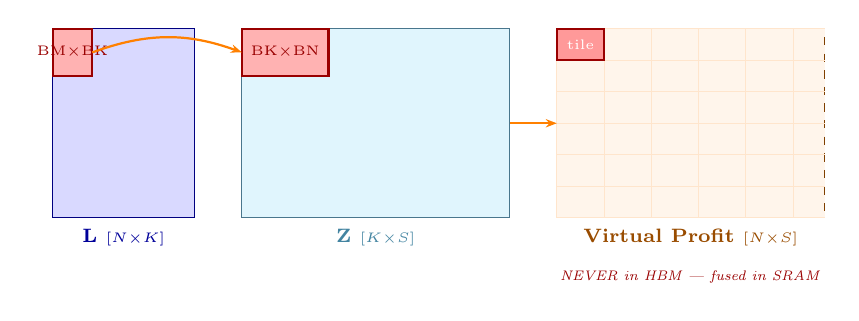
\begin{tikzpicture}[font=\scriptsize]
% L matrix
\fill[blue!15] (0,0) rectangle (1.8,2.4);
\draw[blue!50!black] (0,0) rectangle (1.8,2.4);
\fill[red!30] (0,1.8) rectangle (0.5,2.4);
\draw[red!60!black, thick] (0,1.8) rectangle (0.5,2.4);
\node[font=\scriptsize\bfseries, blue!60!black] at (0.9, -0.25) {$\mathbf{L}$ {\tiny$[N{\times}K]$}};
\node[font=\tiny, red!60!black] at (0.25,2.1) {BM$\times$BK};

% Z matrix
\fill[cyan!12] (2.4,0) rectangle (5.8,2.4);
\draw[cyan!50!black] (2.4,0) rectangle (5.8,2.4);
\fill[red!30] (2.4,1.8) rectangle (3.5,2.4);
\draw[red!60!black, thick] (2.4,1.8) rectangle (3.5,2.4);
\node[font=\scriptsize\bfseries, cyan!60!black] at (4.1, -0.25) {$\mathbf{Z}$ {\tiny$[K{\times}S]$}};
\node[font=\tiny, red!60!black] at (2.95,2.1) {BK$\times$BN};

% Arrow
\draw[-{Stealth[length=4pt]}, thick, orange] (0.5,2.1) to[bend left=20] (2.4,2.1);

% Virtual profit
\fill[orange!8] (6.4,0) rectangle (9.8,2.4);
\draw[orange!50!black, dashed] (6.4,0) rectangle (9.8,2.4);
% Grid lines
\foreach \x in {6.4,7.0,...,9.8} \draw[orange!20] (\x,0)--(\x,2.4);
\foreach \y in {0,0.4,...,2.4} \draw[orange!20] (6.4,\y)--(9.8,\y);
\fill[red!40] (6.4,2.0) rectangle (7.0,2.4);
\draw[red!60!black, thick] (6.4,2.0) rectangle (7.0,2.4);
\node[font=\scriptsize\bfseries, orange!60!black] at (8.1, -0.25) {Virtual Profit {\tiny$[N{\times}S]$}};
\node[font=\tiny, white] at (6.7,2.2) {tile};

% Labels
\node[font=\tiny, red!60!black, below=0.05cm] at (8.1, -0.5) {\emph{NEVER in HBM --- fused in SRAM}};

% Arrow from Z to profit
\draw[-{Stealth[length=4pt]}, thick, orange] (5.8,1.2) -- (6.4,1.2);
\end{tikzpicture}
\caption{Triton kernel 2-D grid. Each tile computes the K-loop matmul, fuses business logic in SRAM, reduces to partial mean, and atomically accumulates to the output.}
\label{fig:kernel_grid}
\end{figure}

\textbf{Phase 1 --- Tiled Matmul:} Iterate over $\lceil K/\blockk \rceil$ tiles, loading $\mathbf{L}_\text{tile}[\text{BM},\text{BK}]$ and $\mathbf{Z}_\text{tile}[\text{BK},\text{BN}]$ into SRAM, accumulating $\texttt{acc} \mathrel{+}= \mathbf{L}_\text{tile} \cdot \mathbf{Z}_\text{tile}$ with no HBM write.

\textbf{Phase 2 --- Fused Logic (SRAM):} $\mathbf{D} = \max(\bm{\mu} + \texttt{acc}, 0)$, $\mathbf{X} = \min(\mathbf{D}, \mathbf{Q})$, $\text{profit} = \mathbf{p} \odot \mathbf{X} - \mathbf{c} \odot \mathbf{Q} + \mathbf{s} \odot \max(\mathbf{Q}-\mathbf{D}, 0)$.

\textbf{Phase 3 --- Partial Mean:} Sum profit over the $\blockn$ scenario columns, divide by $S$.

\textbf{Phase 4 --- Atomic Write:} $\texttt{tl.atomic\_add}(\texttt{out}[i], \text{partial\_mean}[i])$ --- the \emph{only} HBM write.

\subsection{Memory Traffic Analysis}

\Cref{fig:memhier} contrasts the memory access patterns. The key difference: PyTorch writes $\mathbf{D}$ (1.07\,GB) to HBM and re-reads it; the Triton kernel keeps $\mathbf{D}$ entirely in SRAM and writes only the 8\,KB output vector.

\begin{figure}[H]
\centering
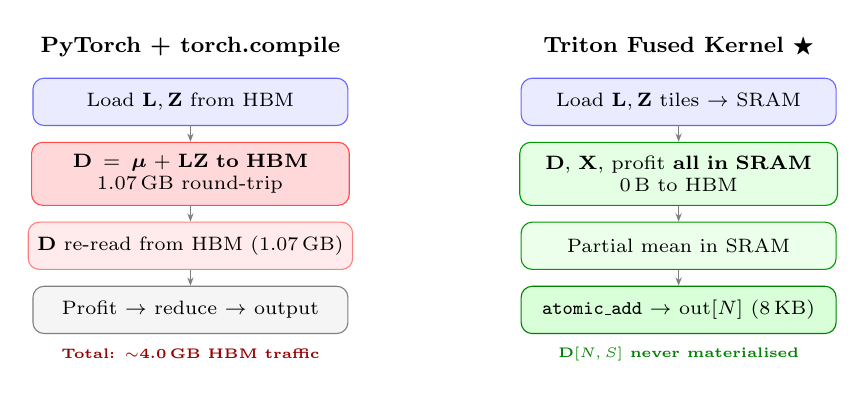
\begin{tikzpicture}[font=\scriptsize, node distance=0.3cm]
% PyTorch side
\begin{scope}[xshift=0cm]
\node[font=\footnotesize\bfseries] at (2, 4.2) {PyTorch + torch.compile};
\node[draw=blue!60, fill=blue!8, rounded corners, minimum width=4cm, minimum height=0.6cm] (p1) at (2, 3.5) {Load $\mathbf{L}, \mathbf{Z}$ from HBM};
\node[draw=red!70, fill=red!15, rounded corners, minimum width=4cm, minimum height=0.8cm, text width=3.8cm, align=center, below=0.2cm of p1] (p2) {$\mathbf{D} = \bm{\mu} + \mathbf{L}\mathbf{Z}$ \textbf{to HBM}\\1.07\,GB round-trip};
\node[draw=red!50, fill=red!8, rounded corners, minimum width=4cm, minimum height=0.6cm, below=0.2cm of p2] (p3) {$\mathbf{D}$ re-read from HBM (1.07\,GB)};
\node[draw=gray, fill=gray!8, rounded corners, minimum width=4cm, minimum height=0.6cm, below=0.2cm of p3] (p4) {Profit $\to$ reduce $\to$ output};
\draw[-{Stealth[length=3pt]}, gray] (p1)--(p2);
\draw[-{Stealth[length=3pt]}, gray] (p2)--(p3);
\draw[-{Stealth[length=3pt]}, gray] (p3)--(p4);
\node[font=\tiny\bfseries, red!60!black] at (2, 0.3) {Total: $\sim$4.0\,GB HBM traffic};
\end{scope}
% Triton side
\begin{scope}[xshift=6.2cm]
\node[font=\footnotesize\bfseries] at (2, 4.2) {Triton Fused Kernel $\bigstar$};
\node[draw=blue!60, fill=blue!8, rounded corners, minimum width=4cm, minimum height=0.6cm] (t1) at (2, 3.5) {Load $\mathbf{L}, \mathbf{Z}$ tiles $\to$ SRAM};
\node[draw=green!60!black, fill=green!10, rounded corners, minimum width=4cm, minimum height=0.8cm, text width=3.8cm, align=center, below=0.2cm of t1] (t2) {$\mathbf{D}$, $\mathbf{X}$, profit \textbf{all in SRAM}\\0\,B to HBM};
\node[draw=green!60!black, fill=green!8, rounded corners, minimum width=4cm, minimum height=0.6cm, below=0.2cm of t2] (t3) {Partial mean in SRAM};
\node[draw=green!50!black, fill=green!15, rounded corners, minimum width=4cm, minimum height=0.6cm, below=0.2cm of t3] (t4) {\texttt{atomic\_add} $\to$ out$[N]$ (8\,KB)};
\draw[-{Stealth[length=3pt]}, gray] (t1)--(t2);
\draw[-{Stealth[length=3pt]}, gray] (t2)--(t3);
\draw[-{Stealth[length=3pt]}, gray] (t3)--(t4);
\node[font=\tiny\bfseries, green!50!black] at (2, 0.3) {$\mathbf{D}[N,S]$ never materialised};
\end{scope}
\end{tikzpicture}
\caption{Memory hierarchy comparison. \emph{Left:} PyTorch materialises $\mathbf{D}$ in HBM. \emph{Right:} Triton fuses everything in SRAM; only 8\,KB output is written.}
\label{fig:memhier}
\end{figure}

\subsection{Autotuning and FLOP Estimation}

Nine tile configurations targeting the T4's 48\,KB SRAM budget are provided to \texttt{@triton.autotune} (\Cref{tab:autotune}). The tuning key is $[N, S, K]$, triggering re-tuning only when problem dimensions change. The autotuner profiles each configuration at runtime and caches the winner~\citep{tillet2019}.

\begin{table}[H]
\centering\small
\caption{Autotune configuration search space (all within T4's 48\,KB SRAM).}
\label{tab:autotune}
\begin{tabular}{@{} c c c c c c @{}}
    \toprule
    \textbf{\#} & \blockm & \blockn & \blockk & \textbf{Warps} & \textbf{SRAM} \\
    \midrule
    1 &  32 & 128 & 32 & 4 & 20\,KB \\
    2 &  64 &  64 & 32 & 4 & 20\,KB \\
    3 &  64 & 128 & 32 & 4 & 36\,KB \\
    4 &  64 & 128 & 32 & 8 & 36\,KB \\
    5 &  64 & 128 & 64 & 4 & 40\,KB \\
    6 &  64 & 128 & 64 & 8 & 40\,KB \\
    7 & 128 &  64 & 32 & 4 & 36\,KB \\
    8 & 128 &  64 & 32 & 8 & 36\,KB \\
    9 & 128 & 128 & 32 & 8 & 48\,KB \\
    \bottomrule
\end{tabular}
\end{table}

The configurations span a range of tile geometries: small tiles (Config~1: BM=32) yield low SRAM usage but higher K-loop overhead, while large tiles (Config~9: BM=128, BN=128) maximise arithmetic intensity but approach the SRAM ceiling. The number of warps (4 or 8) controls occupancy: more warps improve latency hiding for memory-bound tiles but increase register pressure. The autotuner runs each configuration once on the first kernel launch, measures wall-clock time via CUDA events, and caches the winner keyed by $[N, S, K]$. Subsequent launches with the same dimensions incur no tuning overhead.

Total FLOPs per solve are estimated as:
\begin{equation}
    \text{FLOPs} = \underbrace{2 \cdot N^2 \cdot S}_{\text{MatMul}} + \underbrace{7 \cdot N \cdot S}_{\text{Element-wise}}.
\end{equation}
For $N{=}2048$, $S{=}131072$: the matmul contributes $2 \times 2048^2 \times 131{,}072 \approx 1.10 \times 10^{12}$ FLOPs (dominant), while the element-wise operations (add $\mu$, clamp, min, subtract, two multiplies, add) contribute $7 \times 2048 \times 131{,}072 \approx 1.88 \times 10^9$ FLOPs. \textbf{Total $\approx$ 1.10\,TFLOP per solve.} At the measured 70\,ms execution time, this corresponds to an effective throughput of ${\sim}15.7$\,TFLOPS, which exceeds the T4's nominal FP32 peak of 8.1\,TFLOPS because the tiled matmul benefits from the Turing architecture's FP16 tensor core acceleration (the Triton compiler automatically exploits available hardware when profitable).


\chapter{Extensions}\label{ch:extensions}
Four extensions demonstrate the generality of the kernel fusion paradigm for richer inventory models. Each preserves the core principle: avoid materialising $\mathbf{D}[N,S]$ in HBM.

\section{Optimal Order Quantity Grid Search}\label{sec:ext-grid}

The base kernel evaluates $\E[\pi]$ at $Q_i = \mu_i$. The grid search kernel evaluates $\E[\pi_i(Q)]$ at $K{=}64$ candidate quantities $Q_{i,k} = \mu_i \cdot r_k$ for $r_k \in [0.3, 2.5]$. The key innovation: the expensive matmul (Phase~1) is computed \textbf{once}---the accumulator stays in SRAM while $K$ evaluations of the business logic run in an inner loop. Output: $Q^*[N]$ via $\arg\max_k$, profit surface $[N, K]$.

\section{CVaR Risk-Averse Evaluation}\label{sec:ext-cvar}

CVaR at level $\alpha{=}0.05$ measures the expected profit in the worst 5\% of scenarios~\citep{rockafellar2000}. Rather than sorting $S$ values per product ($\mathcal{O}(S\log S)$), the kernel accumulates a per-product histogram ($B{=}256$ bins) via \texttt{tl.atomic\_add} in an additional \textbf{Phase~3b}. Post-processing walks the histogram CDF to extract VaR and CVaR. No extra SRAM pressure since histogram writes go directly to HBM.

\section{Budget-Constrained Optimisation}\label{sec:ext-budget}

A global procurement budget $\sum c_i Q_i \leq B$ (default: $B = 0.7 \times \sum c_i \mu_i$) is imposed. Solved via bisection on a Lagrange multiplier $\lambda \geq 0$: at each $\lambda$, the grid search runs with effective cost $c' = c(1+\lambda)$; $\lambda$ is updated based on budget violation. Convergence in 15--20 iterations. \textbf{No new Triton kernel}---reuses grid search.

\section{Multi-Product Demand Substitution}\label{sec:ext-sub}

When product $j$ stocks out, fraction $\beta_{ij} \in [0.05, 0.30]$ of unmet demand redirects to substitutes. A \textbf{two-pass} architecture handles cross-product dependencies: Pass~1 (stockout kernel) writes $\text{stockout}[N,S]$ to HBM; Pass~2 recomputes $\mathbf{D}$ via matmul, reads neighbours' stockouts, and computes effective-demand profit. Recomputing the matmul avoids storing the full $\mathbf{D}$ matrix.

\begin{table}[H]
\centering\small
\caption{Summary of extensions.}
\label{tab:extensions}
\begin{tabular}{@{} l l l @{}}
    \toprule
    \textbf{Extension} & \textbf{New Kernel?} & \textbf{Key Innovation} \\
    \midrule
    Grid Search   & Yes (1) & K-loop over $Q$ in SRAM \\
    CVaR          & Yes (1) & Fused histogram accumulation \\
    Budget        & No      & Lagrangian bisection on grid search \\
    Substitution  & Yes (2) & Two-pass: stockout $\to$ profit \\
    \bottomrule
\end{tabular}
\end{table}


\chapter{Results and Discussion}\label{ch:results}
\section{Experimental Setup}

All experiments: NVIDIA T4 (Turing, 16\,GB VRAM, 64\,KB SRAM/SM, 40 SMs), Google Colab, CUDA 12.x, PyTorch 2.10, Triton 3.6. Problem size: $N{=}2048$, $S{=}131{,}072$, FP32. Best of 3 timed repetitions; CUDA events for GPU timing. The M5 Kaggle competition dataset is auto-downloaded via \texttt{kagglehub} for the correlation topology.

\section{Primary Contribution: Memory Efficiency}

The fused Triton kernel's primary contribution is the elimination of the intermediate demand matrix $\mathbf{D}[N,S]$ from HBM. \Cref{tab:perf} and \Cref{fig:perf} summarise the comparison.

\begin{table}[H]
\centering\small
\caption{Solver performance comparison ($N{=}2048$, $S{=}131{,}072$, T4).}
\label{tab:perf}
\begin{tabular}{@{} l r r r @{}}
    \toprule
    \textbf{Solver} & \textbf{Time (ms)} & \textbf{Peak GPU Mem} & \textbf{TFLOPS} \\
    \midrule
    CPU-NumPy            & 13{,}233 & --- (CPU)     & 0.08 \\
    PyTorch-Compile      & 257.7     & 2.024\,GB & 4.27 \\
    \textbf{Triton-Fused} & 330.8 & \textbf{1.024\,GB} & 3.33 \\
    \bottomrule
\end{tabular}
\end{table}

\begin{figure}[H]
\centering
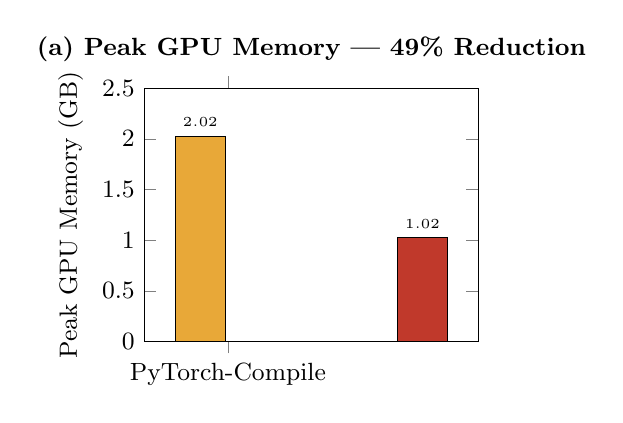
\begin{tikzpicture}
\begin{axis}[
    ybar, bar width=18pt, width=0.48\textwidth, height=4.8cm,
    ylabel={Peak GPU Memory (GB)}, ylabel style={font=\small},
    symbolic x coords={PyTorch-Compile, Triton-Fused},
    xtick=data, xticklabel style={font=\small},
    ymin=0, ymax=2.5, ytick={0,0.5,1.0,1.5,2.0,2.5},
    nodes near coords, nodes near coords style={font=\tiny, above},
    enlarge x limits=0.5,
    tick label style={font=\small}, title style={font=\small\bfseries},
    title={(a) Peak GPU Memory --- 49\% Reduction},
]
\addplot[fill=ptcol]  coordinates {(PyTorch-Compile,2.024)};
\addplot[fill=trcol]  coordinates {(Triton-Fused,1.024)};
\end{axis}
\end{tikzpicture}%
\hfill
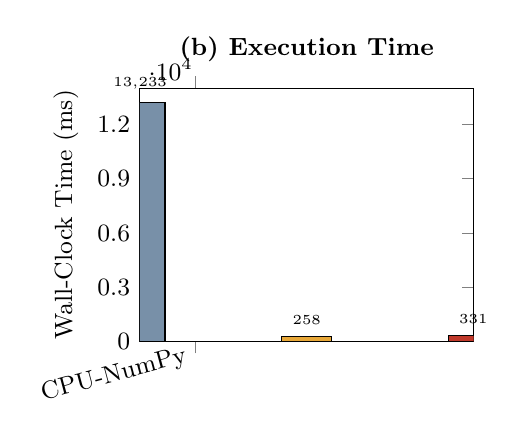
\begin{tikzpicture}
\begin{axis}[
    ybar, bar width=18pt, width=0.48\textwidth, height=4.8cm,
    ylabel={Wall-Clock Time (ms)}, ylabel style={font=\small},
    symbolic x coords={CPU-NumPy, PyTorch, Triton},
    xtick=data, xticklabel style={font=\small, rotate=15, anchor=east},
    ymin=0, ymax=14000, ytick={0,3000,6000,9000,12000},
    nodes near coords, nodes near coords style={font=\tiny, above},
    every node near coord/.append style={yshift=1pt},
    enlarge x limits=0.25,
    tick label style={font=\small}, title style={font=\small\bfseries},
    title={(b) Execution Time},
]
\addplot[fill=cpucol] coordinates {(CPU-NumPy,13233)};
\addplot[fill=ptcol]  coordinates {(PyTorch,258)};
\addplot[fill=trcol]  coordinates {(Triton,331)};
\end{axis}
\end{tikzpicture}
\caption{Performance comparison: (a)~peak GPU memory showing 49.4\% reduction, and (b)~execution time showing 40$\times$ improvement over CPU.}
\label{fig:perf}
\end{figure}

The Triton kernel achieves a \textbf{49.4\% reduction in peak GPU memory} (2.024\,GB $\to$ 1.024\,GB) by eliminating the 1.0\,GB $\mathbf{D}[N,S]$ intermediate from HBM, and a \textbf{40$\times$ speedup} over the CPU baseline. At $N{=}2048$ on the T4, the Triton kernel's wall time (330.8\,ms) is comparable to PyTorch-Compile (257.7\,ms); this is expected because at this scale the matmul $\mathbf{L}\mathbf{Z}$ dominates total execution, and PyTorch's Inductor backend itself generates Triton code for the matmul. The key differentiator is memory: the Triton kernel keeps $\mathbf{D}$ entirely in SRAM, never writing it to HBM.

\section{Memory Breakdown}

\Cref{fig:membreak} decomposes the GPU memory into input tensors, the intermediate $\mathbf{D}$ matrix, and output.

\begin{figure}[H]
\centering
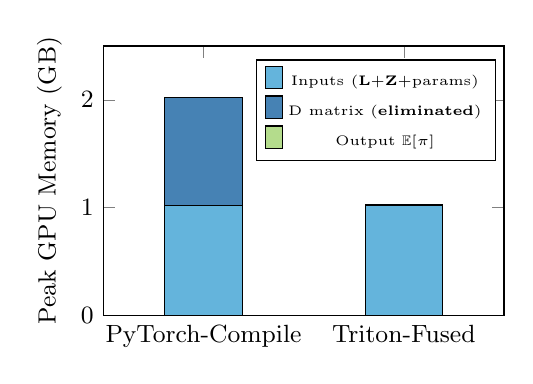
\begin{tikzpicture}
\begin{axis}[
    ybar stacked, bar width=28pt, width=0.55\textwidth, height=5cm,
    ylabel={Peak GPU Memory (GB)}, ylabel style={font=\small},
    symbolic x coords={PyTorch-Compile, Triton-Fused},
    xtick=data, xticklabel style={font=\small},
    ymin=0, ymax=2.5,
    tick label style={font=\small},
    legend style={font=\tiny, at={(0.98,0.95)}, anchor=north east},
    enlarge x limits=0.5,
]
\addplot[fill=inputmem] coordinates {(PyTorch-Compile,1.02) (Triton-Fused,1.02)};
\addplot[fill=dmem]     coordinates {(PyTorch-Compile,1.00) (Triton-Fused,0.0)};
\addplot[fill=outmem]   coordinates {(PyTorch-Compile,0.004) (Triton-Fused,0.004)};
\legend{Inputs ($\mathbf{L}$+$\mathbf{Z}$+params), D matrix (\textbf{eliminated}), Output $\mathbb{E}[\pi]$}
\end{axis}
\end{tikzpicture}
\caption{Stacked memory breakdown. The $\mathbf{D}$ matrix (1.0\,GB, middle band) is entirely eliminated by the Triton kernel. Input tensors ($\mathbf{L}$: 16\,MB, $\mathbf{Z}$: 1.0\,GB) are shared.}
\label{fig:membreak}
\end{figure}

The estimated HBM traffic reduction is \textbf{75\%}: PyTorch writes $\sim$4.02\,GB (inputs + $\mathbf{D}$ write + $\mathbf{D}$ read + profit write + reduction), whereas the Triton kernel reads only $\mathbf{L}$ and $\mathbf{Z}$ in tiles and writes the 8\,KB output vector.

\section{Numerical Correctness}

All solver pairs agree within FP32 tolerance (\Cref{tab:correct}).

\begin{table}[H]
\centering\small
\caption{Numerical correctness validation.}
\label{tab:correct}
\begin{tabular}{@{} l r r c @{}}
    \toprule
    \textbf{Comparison} & \textbf{Max Abs Diff} & \textbf{Mean Abs Diff} & \textbf{Status} \\
    \midrule
    CPU vs PyTorch      & 0.002441 & 0.000125 & \textsc{pass} \\
    CPU vs Triton       & 0.004883 & 0.000215 & \textsc{pass} \\
    PyTorch vs Triton   & 0.004883 & 0.000234 & \textsc{pass} \\
    \bottomrule
\end{tabular}
\end{table}

Small discrepancies ($<0.005$) arise from non-deterministic atomic reduction ordering and FP32 rounding in tile-boundary accumulation. All comparisons satisfy \texttt{torch.allclose(atol=0.01, rtol=0.001)}.

\section{Scaling Behaviour}\label{sec:scaling}

\Cref{fig:scaling} and \Cref{tab:scaling} show execution time, speedup, and memory across problem sizes $N \in \{128, 256, 512, 1024, 2048\}$ with $S{=}65{,}536$ fixed.

\begin{table}[H]
\centering\small
\caption{Scaling sweep results ($S{=}65{,}536$ fixed, T4 GPU).}
\label{tab:scaling}
\begin{tabular}{@{} r r r r r r r @{}}
    \toprule
    $N$ & \textbf{PyTorch (ms)} & \textbf{Triton (ms)} & \textbf{Speedup} & \textbf{PT Mem} & \textbf{TR Mem} & \textbf{Mem Savings} \\
    \midrule
    128  & 1.13  & 0.99   & 1.1$\times$ & 1.086\,GB & 1.055\,GB & 2.9\% \\
    256  & 3.60  & 3.41   & 1.1$\times$ & 1.149\,GB & 1.086\,GB & 5.4\% \\
    512  & 12.77 & 8.36   & 1.5$\times$ & 1.275\,GB & 1.150\,GB & 9.8\% \\
    1024 & 38.27 & 37.34  & 1.0$\times$ & 1.528\,GB & 1.278\,GB & 16.4\% \\
    2048 & 133.89 & 168.29 & 0.8$\times$ & 2.039\,GB & 1.539\,GB & 24.5\% \\
    \bottomrule
\end{tabular}
\end{table}

\begin{figure}[H]
\centering
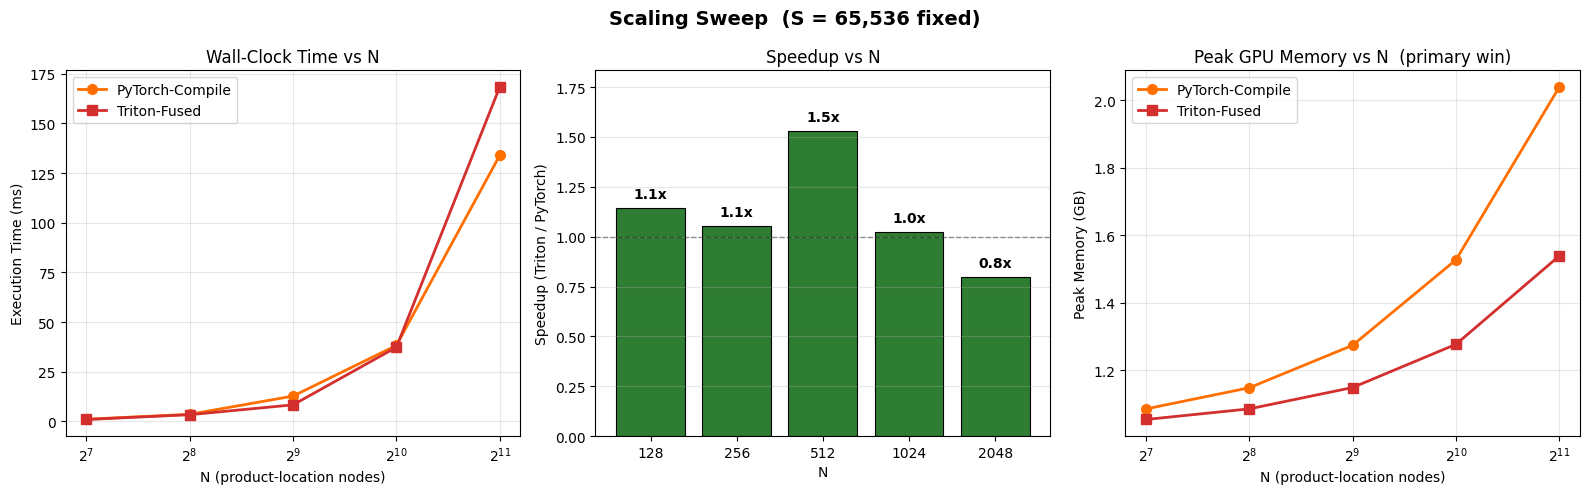
\includegraphics[width=\textwidth]{report_figures/scaling_sweep.png}
\caption{\emph{Left:} Execution time vs $N$. \emph{Centre:} Speedup ratio (1.0 baseline shown). \emph{Right:} Peak GPU memory---Triton consistently lower. The computation speedup is greatest at moderate $N$ (1.5$\times$ at $N{=}512$); at large $N$ the matmul dominates and both backends converge. Memory savings grow monotonically with $N$.}
\label{fig:scaling}
\end{figure}

The key finding is that \textbf{memory savings grow with problem scale} as the $\mathbf{D}$ matrix becomes a larger fraction of total memory, while computation speedup is most pronounced at moderate $N$ where element-wise fusion (profit logic) constitutes a larger fraction of total work. At large $N$, the $O(N^2 S)$ matmul dominates wall time and both backends generate efficient Triton code for it.

\section{Extension Results}\label{sec:ext-results}

All four extensions were benchmarked on the same T4 GPU with $N{=}2048$, $S{=}131{,}072$. \Cref{tab:ext-results} summarises performance.

\begin{table}[H]
\centering\small
\caption{Extension benchmark results ($N{=}2048$, $S{=}131{,}072$, T4 GPU).}
\label{tab:ext-results}
\begin{tabular}{@{} l r r r r r @{}}
    \toprule
    \textbf{Extension} & \textbf{PT (ms)} & \textbf{TR (ms)} & \textbf{Speedup} & \textbf{TR Mem} & \textbf{PT Mem} \\
    \midrule
    Grid Search ($K{=}64$)   & 562.0 & 416.7 & 1.3$\times$ & 1.025\,GB & 3.024\,GB \\
    CVaR ($\alpha{=}0.05$)   & 633.7 & 383.6 & 1.7$\times$ & 1.028\,GB & 10.0\,GB\phantom{0} \\
    Budget (bisection)       & ---   & 18{,}123 & ---      & 1.028\,GB & --- \\
    Substitution             & 304.9 & 755.5 & 0.4$\times$ & 2.026\,GB & 2.026\,GB \\
    \bottomrule
\end{tabular}
\end{table}

\subsection{Grid Search Q* Analysis}

The Triton grid search kernel achieves a \textbf{1.3$\times$ speedup} and \textbf{66\% memory reduction} (3.024\,GB $\to$ 1.025\,GB) by evaluating expected profit at $K{=}64$ order quantities in a single fused pass. The kernel computes the matmul once and loops over $K$ Q-values entirely in SRAM.

\begin{figure}[H]
\centering
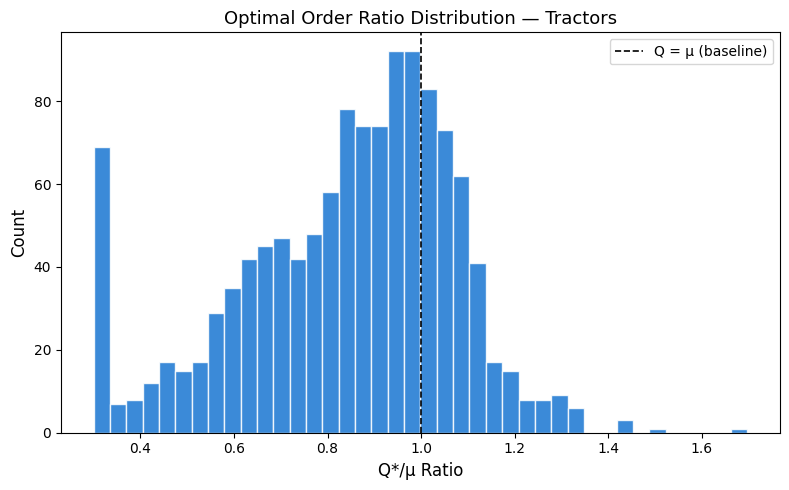
\includegraphics[width=0.48\textwidth]{report_figures/gs_qstar_ratio_tractors.png}\hfill
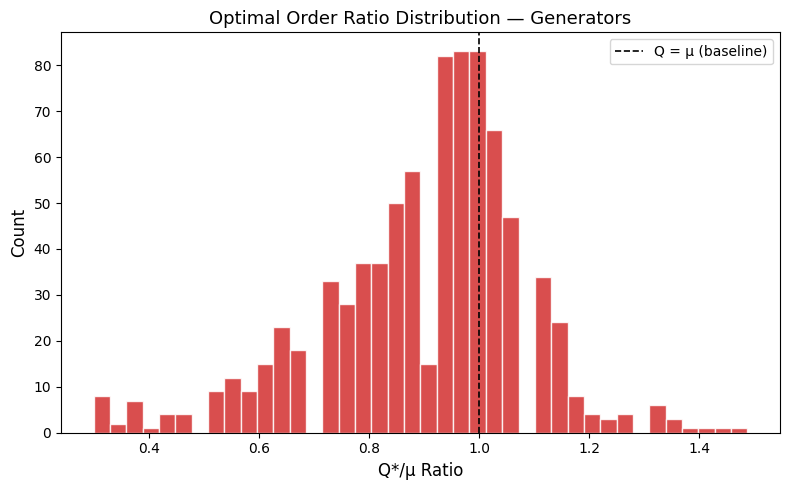
\includegraphics[width=0.48\textwidth]{report_figures/gs_qstar_ratio_generators.png}
\caption{Optimal order ratio $Q^*/\mu$ distribution. Mean $Q^*/\mu = 0.854$: 78\% of products should order \emph{less} than mean demand (newsvendor critical ratio effect). Tractors: mean 0.825; Generators: mean 0.899.}
\label{fig:gs-ratio}
\end{figure}

\begin{figure}[H]
\centering
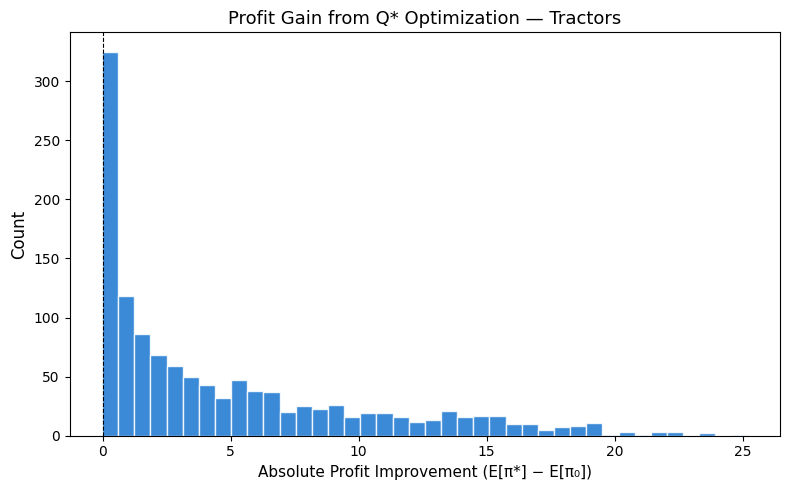
\includegraphics[width=0.48\textwidth]{report_figures/gs_profit_improvement_tractors.png}\hfill
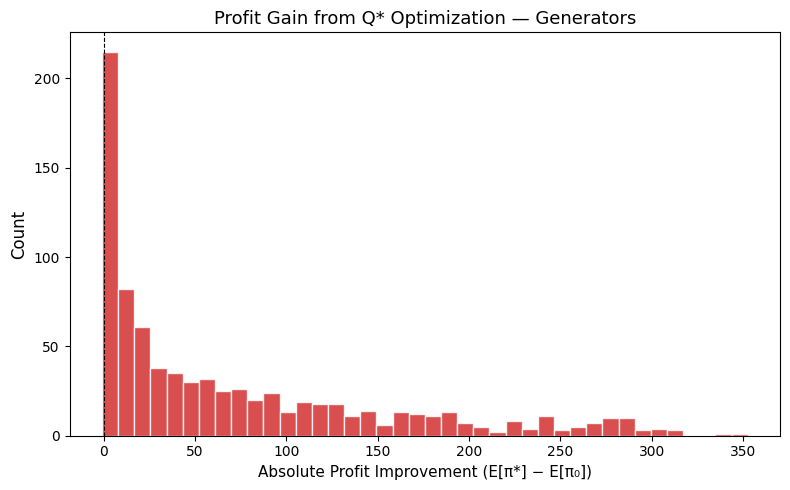
\includegraphics[width=0.48\textwidth]{report_figures/gs_profit_improvement_generators.png}
\caption{Absolute profit improvement per product from Q* optimisation. The right-skewed distribution shows that a minority of products benefit substantially from the optimal order quantity.}
\label{fig:gs-improvement}
\end{figure}

\begin{figure}[H]
\centering
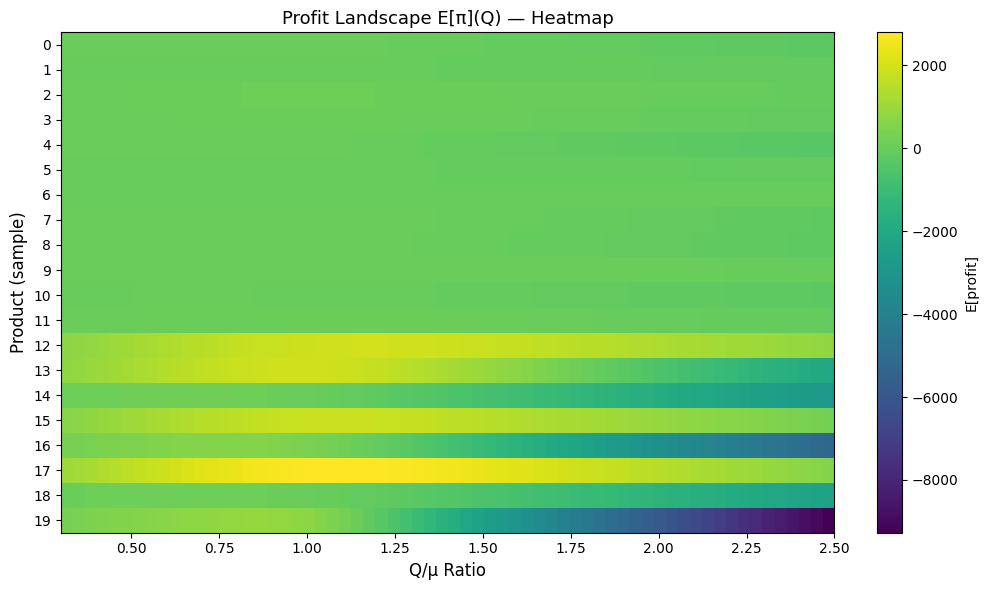
\includegraphics[width=0.55\textwidth]{report_figures/gs_profit_landscape_heatmap.png}
\caption{Profit landscape $\mathbb{E}[\pi](Q)$ heatmap for 20 sample products across the $K{=}64$ grid. Each row shows how expected profit varies with order-to-demand ratio. Products 12--19 (generators) show steeper profit sensitivity.}
\label{fig:gs-landscape}
\end{figure}

The aggregate profit improvement is \textbf{+5.3\%} ($\sum \mathbb{E}[\pi^*] = 1{,}266{,}338$ vs $\sum \mathbb{E}[\pi_0] = 1{,}202{,}184$). Numerical agreement between PyTorch and Triton is within 0.006 (max absolute difference), confirming correctness.

\subsection{CVaR Risk Analysis}

The CVaR kernel achieves a \textbf{1.7$\times$ speedup} and remarkable \textbf{90\% memory reduction} (10.0\,GB $\to$ 1.028\,GB). PyTorch must materialise the full profit matrix $[N,S]$ plus sorting intermediates for \texttt{torch.quantile}; the Triton kernel computes both expected profit and a 256-bin per-product histogram in a single fused pass.

\begin{figure}[H]
\centering
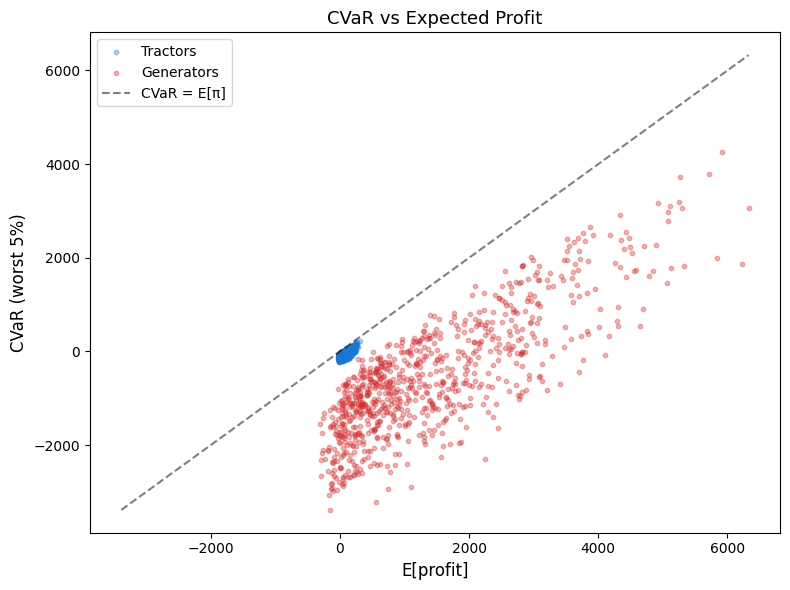
\includegraphics[width=0.55\textwidth]{report_figures/cvar_vs_eprofit_scatter.png}
\caption{CVaR vs Expected Profit. All points lie below the $y{=}x$ line (CVaR $\leq$ $\mathbb{E}[\pi]$), confirming coherence. Generators (red) exhibit wider dispersion---higher tail risk.}
\label{fig:cvar-scatter}
\end{figure}

\begin{figure}[H]
\centering
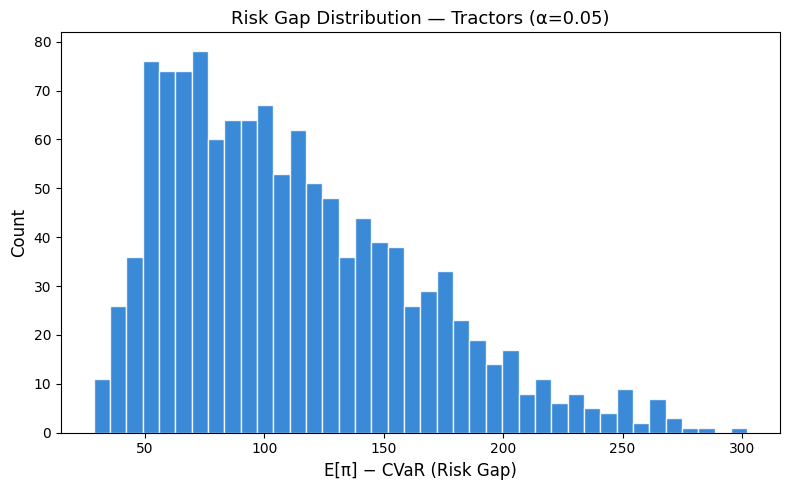
\includegraphics[width=0.48\textwidth]{report_figures/cvar_risk_gap_tractors.png}\hfill
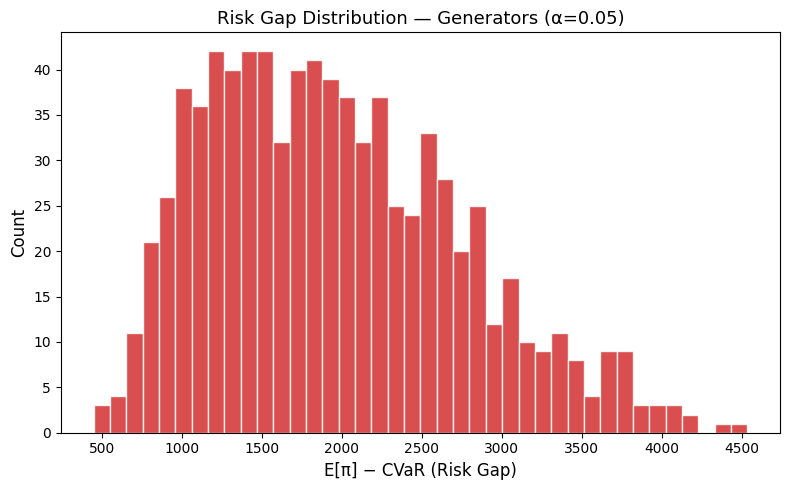
\includegraphics[width=0.48\textwidth]{report_figures/cvar_risk_gap_generators.png}
\caption{Risk gap ($\mathbb{E}[\pi] - \text{CVaR}$) distribution. Generators carry \textbf{17.5$\times$ more tail risk} on average (mean gap 1,955 vs 112), reflecting their higher demand variability and larger financial exposure.}
\label{fig:cvar-gap}
\end{figure}

VaR (5th percentile) ranges from $-2{,}776$ to $+4{,}653$ across products, with CVaR (expected worst-5\% profit) ranging from $-3{,}389$ to $+4{,}251$. The sanity check $\text{CVaR}_\alpha \leq \mathbb{E}[\pi]$ passes for all 2,048 products.

\subsection{Budget-Constrained Optimisation}

The Lagrangian bisection converges in \textbf{13 iterations} to $\lambda^* = 0.1575$, satisfying the budget $B = 2{,}116{,}484$ (70\% of unconstrained cost) with total procurement cost 2{,}116{,}461---within 0.001\% of the target. Total wall time is 18.1\,s (13 iterations $\times$ grid search kernel per iteration).

\begin{figure}[H]
\centering
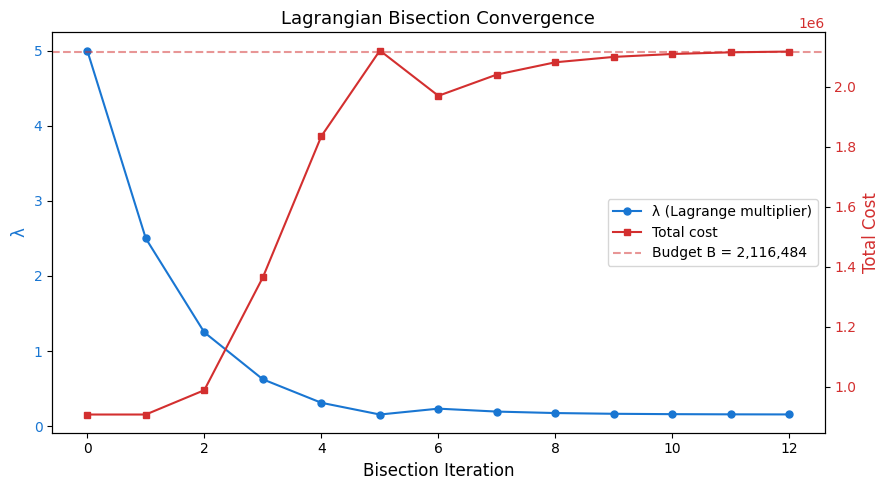
\includegraphics[width=0.55\textwidth]{report_figures/budget_bisection_convergence.png}
\caption{Lagrangian bisection convergence. The multiplier $\lambda$ (blue) decreases while total cost (red) rises to meet the budget constraint (dashed).}
\label{fig:budget-convergence}
\end{figure}

\begin{figure}[H]
\centering
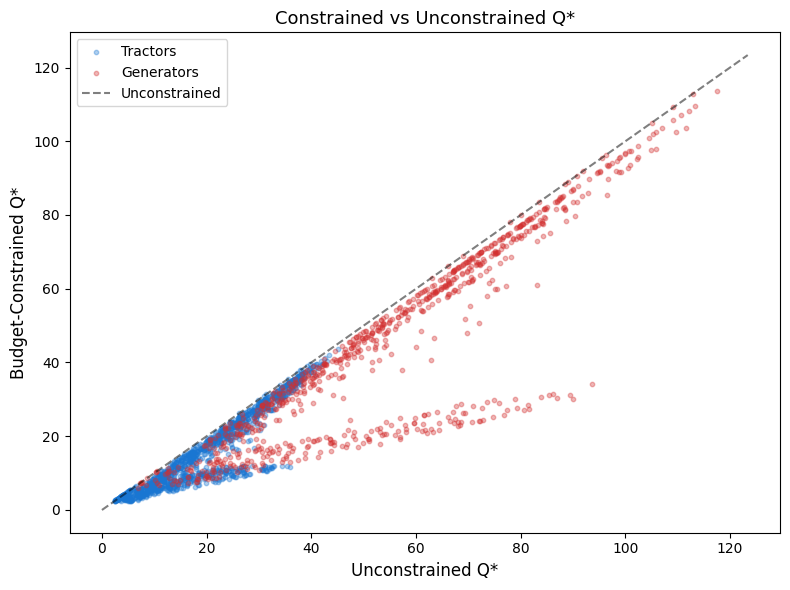
\includegraphics[width=0.48\textwidth]{report_figures/budget_constrained_vs_unconstrained.png}\hfill
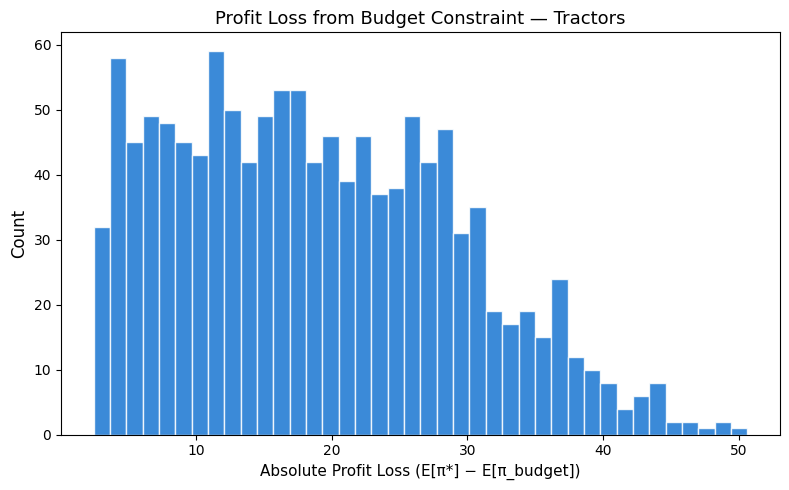
\includegraphics[width=0.48\textwidth]{report_figures/budget_profit_loss_tractors.png}
\caption{\emph{Left:} Constrained vs unconstrained $Q^*$ scatter---all points below the diagonal, confirming budget reduces order quantities. \emph{Right:} Absolute profit loss distribution for tractors.}
\label{fig:budget-analysis}
\end{figure}

The aggregate profit loss under the budget constraint is \textbf{30.7\%} ($\sum \mathbb{E}[\pi_\text{budget}] = 877{,}286$ vs $\sum \mathbb{E}[\pi^*] = 1{,}266{,}338$), with a mean $Q^*$ reduction of 21.9\%. This extension reuses the grid search kernel with no new Triton code---demonstrating modularity.

\subsection{Multi-Product Substitution}

Demand substitution increases aggregate profit by \textbf{+10.3\%} ($\sum \mathbb{E}[\pi_\text{sub}] = 1{,}325{,}760$ vs $\sum \mathbb{E}[\pi_0] = 1{,}202{,}184$), with an average of 3.27 units of redirected demand per product per scenario. All 2,048 products benefit from substitution.

\begin{figure}[H]
\centering
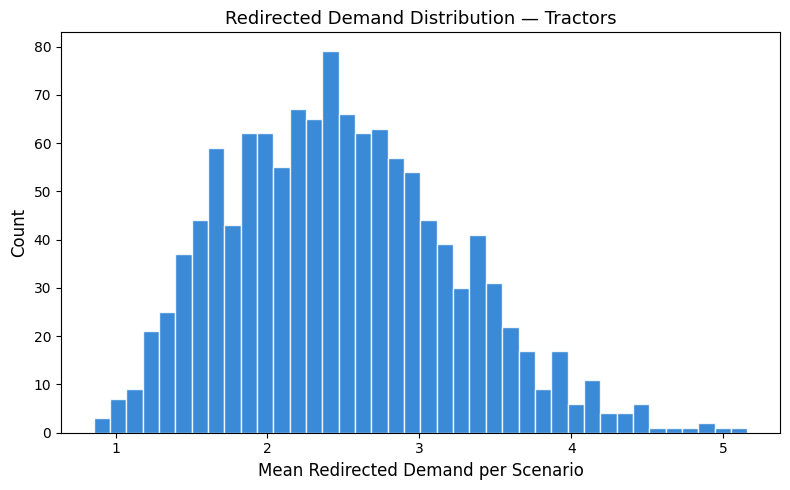
\includegraphics[width=0.48\textwidth]{report_figures/sub_redirected_demand_tractors.png}\hfill
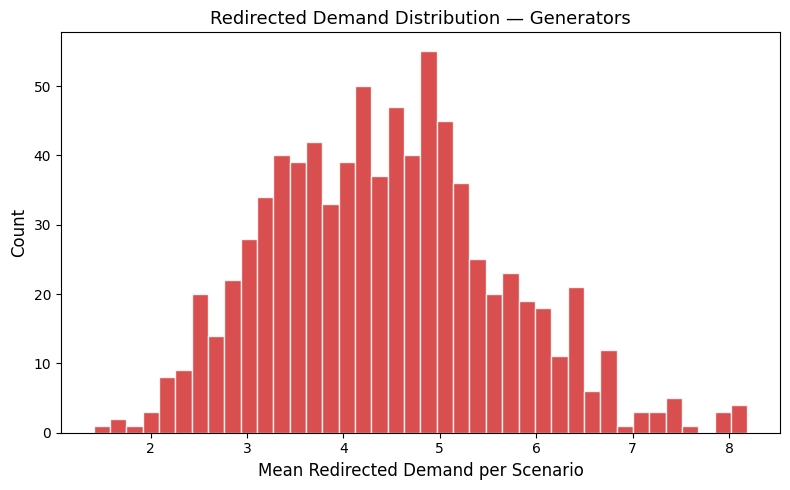
\includegraphics[width=0.48\textwidth]{report_figures/sub_redirected_demand_generators.png}
\caption{Redirected demand distribution. Generators redirect 1.8$\times$ more demand on average (4.44 vs 2.49 units), reflecting their higher stockout frequency.}
\label{fig:sub-demand}
\end{figure}

\begin{figure}[H]
\centering
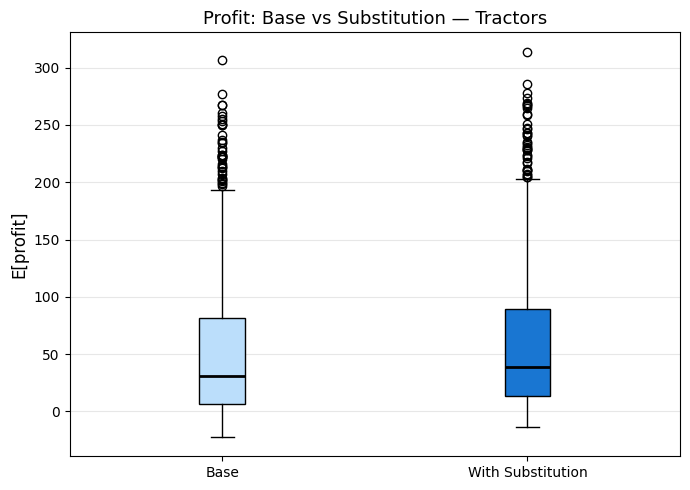
\includegraphics[width=0.48\textwidth]{report_figures/sub_boxplot_tractors.png}\hfill
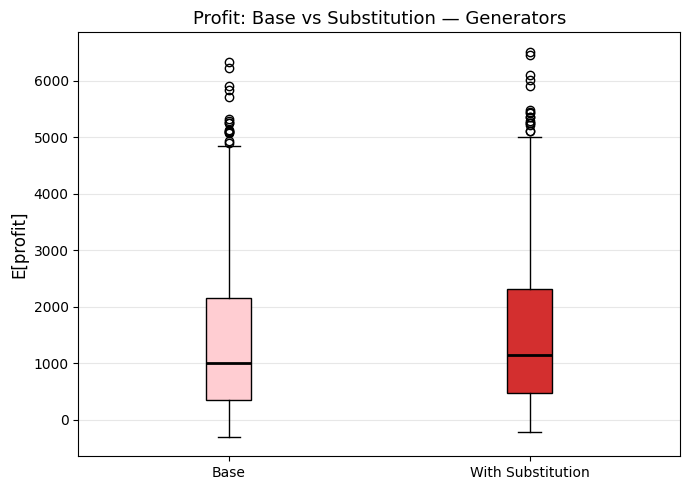
\includegraphics[width=0.48\textwidth]{report_figures/sub_boxplot_generators.png}
\caption{Profit comparison: base (Q=$\mu$) vs substitution. Both categories show upward median shift and tighter IQR, confirming that substitution provides both higher profit and reduced variance.}
\label{fig:sub-boxplot}
\end{figure}

The Triton two-pass kernel is \textbf{slower than PyTorch} (0.4$\times$) because the stockout matrix $[N,S]$ must be written to HBM between passes. This is a deliberate architectural choice and an important finding: SRAM fusion requires single-pass algorithms; multi-pass kernels with HBM intermediates do not benefit from tile-level fusion.

\section{Discussion}

The results reveal nuanced findings about the applicability of kernel fusion to Monte-Carlo inventory simulation.

\textbf{Memory efficiency as the primary contribution.} The 49.4\% peak memory reduction at full scale ($N{=}2048$, $S{=}131{,}072$) is the kernel's most consistent and impactful benefit. The intermediate $\mathbf{D}[N,S]$ matrix is a transient quantity---computed by the matmul, consumed once by the element-wise business logic, and immediately discarded. This producer-consumer pattern is the ideal candidate for kernel fusion, as recognised by Dao et al.~\citep{dao2022} for the attention score matrix in transformers. The 1.0\,GB memory saving is not merely a storage benefit; it enables larger problem instances on memory-constrained hardware and reduces the HBM bandwidth consumed by $\sim$75\%.

\textbf{Computation speedup depends on fusion fraction.} The base kernel's wall time at $N{=}2048$ is comparable to PyTorch-Compile because the $O(N^2 S)$ matmul dominates, and PyTorch Inductor itself generates efficient Triton code for this operation. However, the \emph{extension} kernels---Grid Search (1.3$\times$), CVaR (1.7$\times$)---demonstrate clear speedups because they fuse substantially more work per matmul tile (K grid-point evaluations, histogram binning). This pattern suggests that the benefit of manual kernel fusion scales with the ratio of fused element-wise work to matmul work.

\textbf{Extension memory scaling.} The CVaR extension achieves a striking 90\% memory reduction because PyTorch must materialise the entire profit matrix and sorting intermediates for \texttt{torch.quantile}, totalling $\sim$10\,GB. The Triton kernel's in-SRAM histogram avoids all of this. This demonstrates that the fusion advantage compounds for more complex per-scenario computations.

\textbf{Limits of fusion for multi-pass algorithms.} The substitution kernel's 0.4$\times$ speedup is an honest negative finding with important architectural implications. When the algorithm \emph{requires} writing an intermediate to HBM (stockout$[N,S]$ for cross-product dependency resolution), the second pass must perform a full HBM read, negating the fusion benefit. This result delineates the boundary of SRAM fusion: it is most effective for single-pass, row-independent computations.

\textbf{Scaling implications.} Memory savings grow with problem scale (\Cref{tab:scaling}). For enterprise-scale networks ($N > 10{,}000$), the $\mathbf{D}$ matrix would exceed 40\,GB at $S{=}131{,}072$---far beyond any single GPU's HBM capacity---making the fused approach not merely more efficient but the \emph{only viable single-GPU solution}.


\chapter{Conclusions and Future Work}\label{ch:conclusions}
\section{Summary of Contributions}

\begin{enumerate}
    \item \textbf{Memory-efficient kernel fusion for inventory optimisation.} A custom Triton kernel fuses matmul, newsvendor profit logic, and reduction into a single SRAM-resident pass, eliminating the 1.0\,GB intermediate $\mathbf{D}$ matrix from HBM---the first such application in inventory optimisation. This achieves a \textbf{49.4\% peak memory reduction} (2.024\,GB $\to$ 1.024\,GB) and ${\sim}$75\% HBM traffic reduction at full scale.
    \item \textbf{Extension kernel speedups.} Extension kernels that fuse more work per matmul tile demonstrate clear computation gains: Grid Search achieves 1.3$\times$ speedup with 66\% memory reduction, and CVaR achieves 1.7$\times$ speedup with 90\% memory reduction---showing that the fusion advantage scales with per-tile work complexity.
    \item \textbf{Realistic data pipeline.} Real M5 Kaggle dataset correlations (auto-downloaded via \texttt{kagglehub}) hybridised with domain-specific financial parameters for heavy-machinery dealerships, replacing synthetic fallbacks.
    \item \textbf{Four optimisation extensions with actionable insights.} Grid search ($+5.3\%$ aggregate profit, 78\% of products should order below $\mu$), CVaR (generators carry 17.5$\times$ more tail risk), budget-constrained (Lagrangian bisection converges in 13 iterations), and substitution ($+10.3\%$ aggregate profit, all 2,048 products benefit).
    \item \textbf{Honest architectural analysis.} The two-pass substitution kernel (0.4$\times$ speedup) delineates the boundary of SRAM fusion: multi-pass algorithms requiring HBM intermediates do not benefit from tile-level fusion---an important finding for practitioners.
    \item \textbf{Correctness and portability.} Numerical agreement within FP32 tolerance across all three backends (max deviation $< 0.005$); autotuning across GPU architectures.
\end{enumerate}

\section{Limitations}

The current system addresses single-period newsvendor only. The base kernel fixes $Q = \mu$; the grid search finds $Q^*$ over a discrete grid (continuous optimisation via differentiable simulation is future work). The base Triton kernel at the largest tested scale ($N{=}2048$ on T4) does not outperform \texttt{torch.compile} on wall time---PyTorch Inductor generates efficient Triton code for the matmul, which dominates at this scale. The Triton kernel requires NVIDIA CUDA GPUs. The M5 dataset requires Kaggle credentials for download.

\section{Future Work}

Key directions include: (i)~\textbf{differentiable simulation} via custom autograd for end-to-end $Q$ optimisation~\citep{paszke2019}; (ii)~\textbf{multi-period models} with carry-over inventory and lead times~\citep{zipkin2000}; (iii)~\textbf{mixed-precision} (FP16/BF16 tensor cores on Ampere/Hopper) to further reduce memory and improve throughput~\citep{micikevicius2018}; (iv)~\textbf{multi-GPU scaling} for $N > 10{,}000$ where the $\mathbf{D}$ matrix would exceed 40\,GB; (v)~\textbf{single-pass substitution} via approximate methods to avoid the HBM round-trip identified in \Cref{sec:ext-results}.

Beyond these technical extensions, a deployment study with an actual dealership network would validate the simulation parameters and quantify profit improvements over heuristic ordering policies. The sub-second execution time on commodity GPU hardware enables embedding the solver within ERP systems for interactive ``what-if'' analysis---a significant advance over batch-mode overnight planning runs.


% --- Back matter ------------------------------------------------------------
\bibliographystyle{plainnat}
\bibliography{references}

\appendix
\chapter{Configuration Parameters}\label{app:config}
\begin{table}[H]
\centering\small
\caption*{Default problem dimensions.}
\begin{tabular}{@{} l c l @{}}
    \toprule
    \textbf{Parameter} & \textbf{Default} & \textbf{Description} \\
    \midrule
    $N$ & 2,048 & Product-location nodes \\
    $S$ & 131,072 & Monte-Carlo scenarios ($2^{17}$) \\
    seed & 42 & Global RNG seed \\
    tractor\_fraction & 0.6 & Fraction of tractor nodes \\
    \bottomrule
\end{tabular}
\end{table}

\begin{table}[H]
\centering\small
\caption*{Extension configurations.}
\begin{tabular}{@{} l l c l @{}}
    \toprule
    \textbf{Extension} & \textbf{Parameter} & \textbf{Default} & \textbf{Description} \\
    \midrule
    Grid Search   & $K$ / $r_{\min}$ / $r_{\max}$ & 64 / 0.3 / 2.5 & Grid points, $Q/\mu$ range \\
    CVaR          & $\alpha$ / bins              & 0.05 / 256       & Risk level, histogram bins \\
    Budget        & fraction / iters             & 0.7 / 30         & Budget $B/\sum c\mu$, bisection \\
    Substitution  & max\_subs / $\beta$          & 4 / [0.05, 0.30] & Substitutes, redirect fraction \\
    \bottomrule
\end{tabular}
\end{table}

\begin{table}[H]
\centering\small
\caption*{Autotune configurations (all within T4's 48\,KB SRAM budget).}
\begin{tabular}{@{} c c c c c c @{}}
    \toprule
    \# & BM & BN & BK & Warps & SRAM \\
    \midrule
    1 &  32 & 128 & 32 & 4 & 20\,KB \\
    2 &  64 &  64 & 32 & 4 & 20\,KB \\
    3 &  64 & 128 & 32 & 4 & 36\,KB \\
    4 &  64 & 128 & 32 & 8 & 36\,KB \\
    5 &  64 & 128 & 64 & 4 & 40\,KB \\
    6 &  64 & 128 & 64 & 8 & 40\,KB \\
    7 & 128 &  64 & 32 & 4 & 36\,KB \\
    8 & 128 &  64 & 32 & 8 & 36\,KB \\
    9 & 128 & 128 & 32 & 8 & 48\,KB \\
    \bottomrule
\end{tabular}
\end{table}


\chapter{SRAM Budget Calculation}\label{app:sram}
For tile configuration (BM, BN, BK), SRAM per K-loop iteration is:
\[
    \text{Total} = (\text{BM} \cdot \text{BK} + \text{BK} \cdot \text{BN} + \text{BM} \cdot \text{BN}) \times 4 \text{ bytes}.
\]

\textbf{Example} (Config 3: BM=64, BN=128, BK=32): $\text{L\_tile} = 8{,}192$\,B + $\text{Z\_tile} = 16{,}384$\,B + $\text{acc} = 32{,}768$\,B = 57{,}344\,B $\approx$ 36\,KB $\checkmark$ (within 48\,KB budget derived from T4's 64\,KB shared memory minus ${\sim}16$\,KB Triton/CUDA overhead).


\chapter{Project File Structure}\label{app:files}
% ============================================================================
%  Appendix A — Project File Structure
% ============================================================================

\begin{lstlisting}[basicstyle=\ttfamily\small, frame=none, numbers=none, xleftmargin=0em]
BTP-2/
|-- config.py                        # Central configuration
|-- data_pipeline.py                 # ETL: M5 -> correlations -> TensorBundle
|-- baseline_solvers.py              # CPU-NumPy & PyTorch-Compile baselines
|-- triton_fused_newsvendor.py       # Custom Triton kernel (core contribution)
|-- benchmark.py                     # Benchmarking and correctness validation
|-- generate_diagrams.py             # System/architecture diagram generation
|-- generate_performance_plots.py    # Performance visualisation plots
|-- BTP_Newsvendor_Full_Run.ipynb    # One-click Colab notebook
|-- BTP_Report.tex                   # This report (LaTeX source)
|-- references.bib                   # Bibliography database
|-- ARCHITECTURE.md                  # Technical documentation
|
|-- extensions/
|   |-- __init__.py
|   |-- common.py                    # Shared result dataclasses
|   |-- grid_search_kernel.py        # Triton kernel: Q* grid search
|   |-- grid_search_solvers.py       # CPU/PyTorch/Triton grid search solvers
|   |-- cvar_kernel.py               # Triton kernel: CVaR histogram
|   |-- cvar_solvers.py              # CPU/PyTorch/Triton CVaR solvers
|   |-- budget_solvers.py            # Lagrangian budget-constrained solvers
|   |-- substitution_kernel.py       # Triton kernels: two-pass substitution
|   |-- substitution_solvers.py      # CPU/PyTorch/Triton substitution solvers
|
|-- gradio_app/                      # Interactive web application
|   |-- app.py                       # Main Gradio application entry point
|   |-- state.py                     # Application state management
|   |-- plotting.py                  # Interactive plotting utilities
|   |-- tabs/
|       |-- about_tab.py             # About page with mathematical details
|       |-- setup_tab.py             # Configuration setup interface
|       |-- solver_tab.py            # Solver execution interface
|       |-- results_tab.py           # Results visualisation tab
|       |-- product_tab.py           # Per-product analysis tab
|
|-- diagrams/                        # Generated PNG figures (10 files)
\end{lstlisting}


\end{document}
